\chapter{Vektorgeometrie\label{chapter-vektorgeometrie}}
\rhead{Vektorgeometrie}
Die in den ersten zwei Kapiteln entwickelte Algebra der Vektoren 
hat als eine ihrer grossen Anwendungen die Vektorgeometrie. Die
Idee der analytischen Geometrie, Punkt mittels Koordinaten als Zahlenpaare
oder Zahlentripel zu codieren und damit der Behandlung mittels
Gleichungssystemen zug"anglich zu machen, wird durch eine
vektorielle Beschreibung noch verallgemeinert und deutlich leistungsf"ahiger.

Andererseits steuert die Geometrie auch viele Konzepte bei, die auf
Vektoren beliebiger Dimension verallgemeinert werden k"onnen. Dazu
geh"ort vor allem das Skalarprodukt, welches sich sogar auf
Funktionen, Polynome und weitere Objekte verallgemeinern l"asst.
In der h"oheren Mathematik entsteht daraus die Theorie der Fourier-Reihen,
der Fourier-Transformation, aber auch Approximationspolynome.

Nicht ganz so erfolgreich wie das Skalarprodukt ist das Vektorprodukt,
welches Fl"acheninhalte von Parallelogrammen und Volumina von Spaten
berechnen helfen kann, aber auch immer dann n"utzlich ist, wenn
zu zwei Vektoren ein senkrecht stehender Vektor gesucht ist. Das
Vektorprodukt ist spezifisch f"ur den dreidimensionalen Raum.

In diesem Kapitel wird zun"achst gezeigt, wie Punkte, Geraden und
Ebenen mit Vektoren beschrieben werden k"onnen, und wie sich damit
bereits einige interessante geometrische Probleme rechnerisch l"osen
lassen. In Abschnitt 3.4 wird das Skalarprodukt eingef"uhrt, welches
f"ur L"angen- und Winkelmessung gebraucht wird. Spiegelungen, orthogonale
Vektoren sowie Kreis und Kugel sind wichtige Anwendungen davon.
Der letzte Abschnitt ist dem Vektorprodukt gewidmet.

\section{Punkte und Koordinatensysteme}
\subsection{Punkte im Raum und Vektoren}
\subsubsection{Koordinatensystem}
Punkte der Ebene k"onnen mit Hilfe eines Koordinatensystems festgelegt
werden: von einem Ausgangspunkt $O$, dem Nullpunkt des Koordinatensystems
aus, werden die Koordinaten entlang zweier aufeinander senkrecht stehender
Richtungen, den Achsrichtungen abgetragen. Die Geraden durch den Ursprung
des Koordinatensystems in Achsrichtung heissen die Koordinatenachsen.

\begin{figure}
\begin{center}
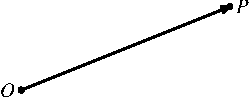
\includegraphics{images/v-1}
\end{center}
\caption{Vektor zwischen zwei Punkten $O$ und $P$, Ortsvektor des Punktes $P$
\label{image-vektor}}
\end{figure}
Ein Punkt $P$ wird durch die L"ange der Projektionen der Strecke $OP$
auf die Achsrichtungen festgelegt, also durch ein Zahlenpaar $(x,y)$.
Der Punkt $(1,0)$ liegt auf der $x$-Achse, eine Einheit vom Punkt $O$
entfernt. Der Punkt $(0,1)$ liegt gleich weit entfernt von $O$ auf der
$y$-Achse.

\subsubsection{Ortsvektoren}
Die Einf"uhrung eines Koordinatensystems erm"oglicht zwar, Punktmengen
in der Ebene durch algebraische Beziehungen zwischen den Koordinaten
zu beschreiben, zum Beispiel ist der Einheitskreis die Menge der
Punkte
\[
\{(x,y)|x^2+y^2=1\}.
\]
``Rechnen'' kann man mit den Punkten aber noch nicht. Dazu bilden wir
die Spaltenvektoren, mit denen wir ja bereits zu rechnen gelernt haben,
wie folgt auf die Punkte der Ebene ab:
\[
\begin{pmatrix}x\\y\end{pmatrix}
\mapsto (x,y)
\]
Den Vektor $\begin{pmatrix}x\\y\end{pmatrix}$ k"onnen wir uns als
Vektor vom Nullpunkt des Koordinatensystems zum Punkt $P=(x,y)$ vorstellen:
\[
\begin{pmatrix}x\\y\end{pmatrix}
=
\overset{\rightarrow}{OP}.
\]
\index{Ortsvektor}
$\overrightarrow{OP}$ heisst
heisst {\em Ortsvektor} des Punktes $P$.
Analoges gilt in drei Dimensionen:
\[
\begin{pmatrix}x\\y\\z\end{pmatrix}
\mapsto
(x,y,z)
\]
Ja es gibt "uberhaupt keinen Grund, die Geometrie auf zwei oder drei
Dimensionen zu beschr"anken, wir k"onnen Vektoren beliebiger Dimension
auf Punkte
abbilden, die entsprechend viele Koordinaten haben:
\[
\begin{pmatrix}
x_1\\x_2\\\vdots\\x_n
\end{pmatrix}
\mapsto
(x_1,x_2,\dots,x_n)
\]

\subsubsection{Vektoroperationen}
Die Rechenoperationen mit Vektoren k"onnen wir ebenfalls in geometrische
Begriffe "ubersetzen:
\begin{figure}
\begin{center}
\begin{tabular}{cc}
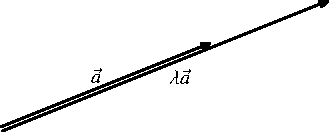
\includegraphics{images/v-2}&
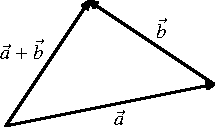
\includegraphics{images/v-3}
\end{tabular}
\end{center}
\caption{Algebraische Operationen mit Vektoren\label{image-vektor-operationen}}
\end{figure}
\begin{itemize}
\index{Streckung}
\item Die Multiplikation mit einer Zahl $\lambda$ ist eine Streckung mit
Zentrum $O$ und Streckfaktor $\lambda$.
\index{Aneinandersetzen}
\item Die Addition von zwei Vektoren entspricht dem ``Aneinandersetzen''
der Strecken.
\end{itemize}
\begin{figure}
\begin{center}
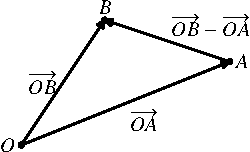
\includegraphics{images/v-4}
\end{center}
\caption{Vektor $\overset{\rightarrow}{AB}$
\label{image-vektorab}}
\end{figure}
Besonders im Falle der Addition spielt die ``Richtung'' der Strecken eine
Rolle, wir symbolisieren diese Richtung durch einen Pfeil. Der Pfeil
vom Punkt $A$ zum Punkt $B$ ist die Differenz der Vektoren die von
$O$ zum Punkt $B$ bzw.~zu $A$ f"uhren:
\[
\overset{\rightarrow}{AB}=\overset{\rightarrow}{OB}-\overset{\rightarrow}{OA}
\]

\subsubsection{Vektoren als Translationen}
Vektoren k"onnen auch als Verschiebungs-Operationen  oder Translationen
des Raumes betrachtet werden.
Wenn eine Verschiebung den Punkt $A$ in den Punkt $B$ verschiebt,
verschiebt sie den Punkt $C$ in den Punkt $D$ mit Ortsvektor
\[
\overrightarrow{OD}
=
\overrightarrow{OC}+\overrightarrow{AB}
=
\overrightarrow{OC}+\overrightarrow{OB}-\overrightarrow{OA}.
\]
Die Verschiebung entspricht also der Addition eines Verschiebungsvektors
zu allen Ortsvektoren.

\subsubsection{Bemerkungen zur Notation}
In diesem geometrischen Zusammenhang werden wir oft Vektoren als
kleine Buchstaben mit einem Pfeil schreiben: $\vec v$. Um jedoch interessante
Geometrie zu treiben, m"ussen wir die "ublichen geometrischen Begriffe in
Vektorschreibweise "ubersetzen: Geraden, Ebenen, Kreise, Kugeln. Ausserdem
m"ussen wir lernen, wie "ubliche geometrische Konstruktionen in 
Rechenoperationen mit Vektoren "ubersetzt werden k"onnen.

\subsection{Basis}
\index{Basis}
\begin{figure}
\begin{center}
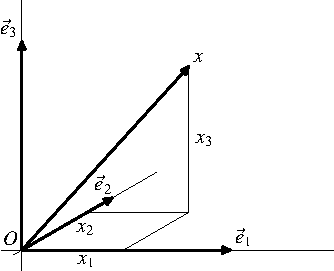
\includegraphics{images/v-5}
\end{center}
\caption{Koordinatensystem und Basis\label{imagebasis}}
\end{figure}
Im Abschnitt \ref{speziellevektoren} haben wir die Vektoren $e_i$
kennengelernt. Im aktuellen Zusammenhang schreiben wir daf"ur oft auch
\[
\vec e_1=\begin{pmatrix}1\\0\\0\end{pmatrix},\qquad
\vec e_2=\begin{pmatrix}0\\1\\0\end{pmatrix},\qquad
\vec e_1=\begin{pmatrix}0\\0\\1\end{pmatrix}.
\]
Diese Vektoren konnten daf"ur verwendet werden, einen beliebigen Vektor
mit Hilfe einer Linearkombination zusammenzusetzen:
\[
\vec v=
v_1\vec e_1+
v_2\vec e_2+
v_3\vec e_3.
\]
Die speziellen Vektoren $e_1,\dots,e_n$ sind nicht die einzig m"oglichen,
mit denen man die Position eines Punktes auf vektorielle Weise
beschreiben k"onnte. Jeder andere Satz von $n$ Vektoren kann
dazu verwendet werden, sofern sich damit jeder beliebige Vektor
linear kombinieren l"asst.  In Kapitel~1 haben wir gelernt, dass dies
gleichbedeutend damit ist, dass die Vektoren linear unabh"angig sein
m"ussen.
\begin{definition}
$n$ linear unabh"angige Vektoren $b_1,\dots,b_n$ heissen eine
Basis des $n$-dimensionalen Raumes.
\end{definition}
Um die Koordinaten eines Punktes $x$ in dieser Basis zu bestimmen,
m"ussen die Zahlen $\xi_1,\dots,\xi_n$ berechnet werden f"ur die
gilt
\[
b_1\xi_1+\dots+b_n\xi_n=x.
\]
Ausgeschrieben ist dies das Gleichungssystem
\[
\begin{linsys}{3}
b_{11}\xi_1&+&\dots &+&b_{1n}\xi_n&=&x_1\\
\vdots   & &\ddots& &\vdots&&\vdots\\
b_{n1}\xi_1&+&\dots &+&b_{nn}\xi_n&=&x_n\\
\end{linsys}
\]
Sind die Vektoren linear unabh"angig, dann ist die Koeffizientenmatrix
regul"ar, das Gleichungssystem hat also genau eine L"osung. Die
behauptete Darstellung ist also immer m"oglich.

Somit haben wir eine weitere Interpretation einer regul"aren Matrix:
die Spalten einer regul"aren Matrix sind Vektoren, die man dazu verwenden
kann, jeden beliebigen anderen Vektor linear zu kombinieren.

\begin{beispiel}
Man stelle den Vektor $\vec v$ in der Basis $b_1,b_2,b_3$ dar:
\[
\vec b_1=\begin{pmatrix}2\\-3\\-2\end{pmatrix},\quad
\vec b_2=\begin{pmatrix}6\\-2\\-3\end{pmatrix},\quad
\vec b_3=\begin{pmatrix}-1\\2\\1\end{pmatrix},\qquad
\vec v=\begin{pmatrix}-6\\3\\3\end{pmatrix}.
\]

\smallskip

{\parindent 0pt
Die} Koordinaten $(\xi_1,\xi_2,\xi_3)$ m"ussen gefunden
werden, so dass
\[
\xi_1\vec b_1+
\xi_2\vec b_2+
\xi_3\vec b_3
=
\vec v,
\]
d.~h.
\[
\xi_1\begin{pmatrix}2\\-3\\-2\end{pmatrix}+
\xi_2\begin{pmatrix}6\\-2\\-3\end{pmatrix}+
\xi_3\begin{pmatrix}-1\\2\\1\end{pmatrix}=
\begin{pmatrix}-6\\3\\3\end{pmatrix}
\quad
\Leftrightarrow
\quad
\begin{pmatrix}
2&6&-1\\
-3&-2&2\\
-2&-3&1
\end{pmatrix}
\begin{pmatrix}\xi_1\\\xi_2\\\xi_3\end{pmatrix}
=
\begin{pmatrix}-6\\3\\3\end{pmatrix}.
\]
Aufl"osung des Gleichungssystems mit dem Gauss-Algorithmus oder mit
dem Computer ergibt.
\[
\begin{pmatrix}\xi_1\\\xi_2\\\xi_3\end{pmatrix}
=
\begin{pmatrix}1\\-1\\2 \end{pmatrix}.
\]
\end{beispiel}

\section{Geraden}
\begin{figure}
\begin{center}
\begin{tabular}{ccc}
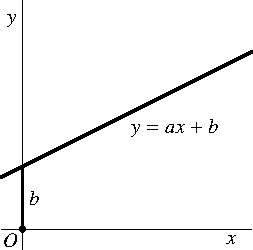
\includegraphics{images/v-6}&%
\qquad\qquad\qquad&
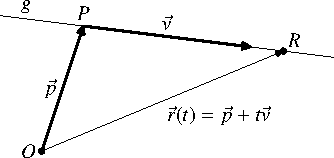
\includegraphics{images/v-7}%
\end{tabular}
\end{center}
\caption{Gerade in der Ebene (links) und Parametrisierung von Geraden im
Raum (rechts) \label{image-gerade}}
\end{figure}
Eine Gerade in einem Koordinatensystem in der Ebene kann durch eine
Gleichung der Form
\[
y=ax+b
\]
beschrieben werden (Abbildung~\ref{image-gerade}).
Die Gleichung hat als L"osungsmenge die Punkte
$(x,y)$, die auf einer Geraden der Steigung $a$ durch den Punkt $(0,b)$
liegen.
Der Nachteil dieser Darstellung ist, dass sich Geraden parallel zur $y$-Achse
damit nicht abbilden lassen. Solche Geraden haben die Gleichung $x=c$, sie haben
``unendlich'' grosse Steigung.
Eine weitere Schwierigkeit besteht im Raum, wo noch eine weiter Koordinate
festzulegen ist. Auch diese ist mit einer einzigen Gleichung nicht m"oglich.
Wir ben"otigen daher eine neue Form der Geradengleichung, welche f"ur beliebige
Geraden in beliebigen Richtungen durch beliebige Punkte in beliebigen R"aumen
unabh"angig von der Dimension funktionieren.

\subsection{Parameterdarstellung}
\index{Parameterdarstellung!einer Gerade}
Die Punkte einer Geraden enstehen dadurch, dass ein Ausgangspunkt um
variable L"angen in immer die gleiche Richtung verschoben wird. Dies "ubersetzen
wird jetzt in die Vektorsprache. Eine Gerade wird also beschrieben durch
\begin{itemize}
\item einen Ausgangspunkt, oder seinen Ortsektor $\vec p$. Dieser Vektor
heisst oft auch {\em St"utzvektor}.
\index{Stutzvektor@St\"utzvektor}
\item Von diesem Ausgangspunkt aus m"ussen Strecken in eine bestimmte
Richtung angesetzt werden, dazu brauchen wir einen Vektor, wir nennen ihn
$\vec v$, den {\em Richtungsvektor}.
\index{Richtungsvektor}
\item Die angesetzten Vektoren sind von variabler L"ange, es braucht also
einen Parameter, den wir $t\in \mathbb R$ nennen, mit welchem $\vec v$
multipliziert wird.
\end{itemize}
Auf diese Weise erreichen wir die Punkte $\vec r$ der Gerade mit Hilfe
einer Addition:
\[
\vec r(t)=\vec p+t\vec v,
\]
Abbildung~\ref{image-gerade}, rechts.
Mit dieser Definition lassen sich gewisse Grundaufgaben bereits l"osen.

\begin{beispiel}
Man finde die Parameterdarstellung der Geraden durch die Punkte
$A=(3,1,4)$ und $B=(1,5,9)$.

\smallskip

{\parindent 0pt
Dazu} braucht man einen Vektor, der die Funktion von $\vec p$ "ubernehmen
kann, wir verwenden $\overrightarrow{OA}$ daf"ur, und als
Richtungsvektor k"onnen wir $\overrightarrow{AB}$ verwenden. Damit wird
die Geradengleichung
\begin{equation}
\vec r(t) =
\begin{pmatrix}3\\1\\4 \end{pmatrix}
+t
\begin{pmatrix}-2\\4\\5\end{pmatrix}.
\label{pigerade}
\end{equation}
\end{beispiel}

\subsubsection{Geht eine Gerade durch einen Punkt?}
Gegeben ist die Gerade durch $\vec p$ mit Richtungsvektor $\vec v$. Geht die
Gerade durch den Punkt $\vec s$? Offenbar m"ussen wir herausfinden, ob es
einen Wert des Parameters $t$ gibt, f"ur den der Geradenpunkt mit $\vec s$
identisch ist, also
\[
\vec s = \vec p + t\vec v.
\]
Diese Vektorgleichung ist genau genommen ein Gleichungssystem f"ur die einzelnen
Komponenten
\[
\begin{pmatrix}
s_1\\s_2\\s_3
\end{pmatrix}
=
\begin{pmatrix}
p_1\\p_2\\p_3
\end{pmatrix}
+t
\begin{pmatrix}
v_1\\v_2\\v_3
\end{pmatrix}
\qquad
\Rightarrow
\qquad
\begin{aligned}
s_1&=p_1+tv_1\\
s_2&=p_2+tv_2\\
s_3&=p_3+tv_3
\end{aligned}
\]
Dieses Gleichungssystem mit drei Gleichungen aber nur einer Unbekannten wird
meistens nicht l"osbar sein. Aber es gilt nat"urlich die "ubliche Alternative
f"ur lineare Gleichungssysteme:
\begin{itemize}
\item Es kann keine L"osungen geben: Dieser Fall tritt ein, wenn die Gerade
an dem Punkt vorbei geht.
\item Es kann unendlich viele L"osungen geben: Dieser Fall tritt ein, wenn
$\vec v=0$ ist und $\vec p=\vec s$. Dann ``bleibt'' der Punkt $\vec r(t)$
immer am Ort $\vec p$, welcher identisch ist mit dem gesuchten Punkt $\vec s$.
\item Es kann genau eine L"osung geben: falls $\vec v\ne 0$ und der Punkt auf der
Geraden liegt, gibt es genau einen Parameterwert, f"ur den der Punkt
getroffen wird.
\end{itemize}
Den Parameterwert im Fall 3 kann man zum Beispiel finden, indem man eine
der Gleichungen ausw"ahlt, in der der $v_i$-Koeffizient nicht $0$ ist
Diese Gleichung l"ost man nach $t$ auf. Falls $v_1\ne 0$ heisst das
\[
t=\frac{s_1-p_1}{v_1}.
\]
Durch Einsetzen in die anderen Gleichungen kann man anschliessen auch "uberpr"ufen,
ob die Gerade tats"achlich durch den Punkt geht.

\begin{beispiel} Welcher der Punkte $U=(5,-3,-1)$ und $V=(7,-7,-7)$
liegt auf der Geraden (\ref{pigerade})?

\smallskip

{\parindent 0pt Um zu testen},
ob die Gerade durch den Punkt mit Ortsvektor $\vec u$
geht, muss man versuchen, die Gleichung
\[
\begin{pmatrix}3\\1\\4 \end{pmatrix}
+t
\begin{pmatrix}-2\\4\\5\end{pmatrix}
=\vec u
\]
zu l"osen. F"ur die beiden Ortsvektoren $\vec u$ und $\vec v$
bedeutet das
\begin{align*}
t_1
\begin{pmatrix}-2\\4\\5\end{pmatrix}
+
\begin{pmatrix}3\\1\\4 \end{pmatrix}
&=
\begin{pmatrix}5\\-3\\-1\end{pmatrix}
&
\qquad
t_2
\begin{pmatrix}-2\\4\\5\end{pmatrix}
+
\begin{pmatrix}3\\1\\4 \end{pmatrix}
&=
\begin{pmatrix}7\\-7\\-7\end{pmatrix}
\\
t_1
\begin{pmatrix}-2\\4\\5\end{pmatrix}
&=
\begin{pmatrix}5\\-3\\-1\end{pmatrix}
-
\begin{pmatrix}3\\1\\4 \end{pmatrix}
=
\begin{pmatrix}2\\-4\\-5 \end{pmatrix}
&
\qquad
t_2
\begin{pmatrix}-2\\4\\5\end{pmatrix}
&=
\begin{pmatrix}7\\-7\\-7\end{pmatrix}
-
\begin{pmatrix}3\\1\\4 \end{pmatrix}
=
\begin{pmatrix}4\\-8\\-11\end{pmatrix}
\\
t_1&=-1,&t_2&:\text{keine L"osung.}
\end{align*}
Es folgt, dass $U$ auf der Geraden liegt, $V$ aber nicht.
\end{beispiel}

\subsubsection{Geschwindigkeitsvektor}
\index{Geschwindigkeitsvektor}
Interpretiert man $t$ als die Zeit, dann bewegt sich ein Punkt auf der Geraden in
einer Sekunde um $\vec v$, dieser Vektor stellt also die Geschwindigkeit
des Punktes dar. Die Parameterdarstellung der Geraden ist also auch eine
Beschreibung einer gleichf"ormigen Bewegung.

\subsubsection{Spezialfall Dimension 2}
In Dimension 2 wird die Geradengleichung zu
\[
\begin{pmatrix}
x\\y
\end{pmatrix}
=
\begin{pmatrix}
x_0\\y_0
\end{pmatrix}
+t
\begin{pmatrix}
v_x\\v_y
\end{pmatrix}
\qquad
\Rightarrow
\qquad
\begin{aligned}
x&=x_0+tv_x\\
y&=y_0+tv_y
\end{aligned}
\]
Falls $v_x\ne 0$ (was gleichbedeutend ist damit, dass die Gerade
nicht parallel zur $y$-Achse ist, kann man die erste Gleichung nach
$t$ aufl"osen:
\[
t = \frac{x-x_0}{v_x}
\]
und in die zweite Gleichung einsetzen:
\[
y=y_0+
\frac{x-x_0}{v_x}v_y
=
y_0+\frac{v_y}{v_x}(x-x_0)
=
y_0-mx_0 +mx
=
mx+(y_0-mx_0)=mx+b
\]
Es entsteht also eine Geradengleichung der Art, wie sie uns schon fr"uher
bekannt war. Der Quotient
$m=\frac{v_y}{v_x}$
ist offenbar die Steigung der Geraden, $y_0-mx_0$ ist der Achsabschnitt.
Die Vektorschreibweise ist jedoch vorteilhaft, weil sie keine der
Koordinaten besonders hervorhebt, und damit auch Spezialf"alle wie
die $y$-Achse besser darstellen kann\footnote{In diesem Spezialfall ist
$v_x=0$, also ist die Steigung $m=\frac{v_y}{v_x}$ nicht definiert.}.

\subsection{Schnittpunkt von zwei Geraden}
\index{Schnittpunkt zweier Geraden}
Seien jetzt zwei Geraden gegeben, also zwei Ausgangspunkte $\vec p_1$ und
$\vec p_2$ und zwei Richtungsvektoren $\vec v_1$ und $\vec v_2$. Haben die
beiden Geraden einen Schnittpunkt?
Jede der Geraden ist durch die Parameterdarstellung
$\vec r=\vec p_1+t\vec v_1$
bzw.~$\vec r=\vec p_2+t\vec v_2$
gegeben. Wir k"onnen nat"urlich nicht annehmen, dass der Schnittpunkt,
wenn es ihn "uberhaupt gibt, von beiden Geraden mit dem gleichen Parameterwert
$t$ erreicht wird. Wir m"ussen also zwei verschiedene Parameterwerte $t$
und $s$ finden, die eingesetzt in die beiden Geradengleichungen zum gleichen
Punkt f"uhren, also:
\[
\vec p_1+t\vec v_1=\vec p_2+s\vec v_2,
\]
oder
\[
t\vec v_1-s\vec v_2=\vec p_2-\vec p_1.
\]
Dies ist ein Gleichungssystem mit zwei Unbekannten, f"ur die Anzahl der L"osungen
gilt wieder die bekannte Alternative:
\begin{itemize}
\item Keine L"osungen: Die Geraden haben keinen Schnittpunkt, in der Ebene 
kann dies zum Beispiel dadurch geschehen, dass die Geraden parallel sind.
Im Raum k"onnen die Geraden auch windschief sein. In drei Dimensionen
erhalten wir drei Gleichungen mit nur einer Unbekannten, dieses System wir
normalerweise nicht l"osbar sein.
\item Unendlich viele L"osungen: die Geraden sind deckungsgleich
\item Genau eine L"osung: es gibt einen wohldefinierten Schnittpunkt.
\end{itemize}
Gel"ost werden kann das Gleichungssystem nat"urlich mit den Standardverfahren
f"ur lineare Gleichungssysteme.

\begin{beispiel}
Man finde den Schnittpunkt der Geraden $g_1$ und $g_2$ mit den
Parameterdarstellungen
\begin{align*}
g_1:
\vec r
&=t\begin{pmatrix}5\\6\\1\end{pmatrix}+\begin{pmatrix}0\\4\\2\end{pmatrix}
&
g_2:
\vec r
&=s\begin{pmatrix}5\\2\\4\end{pmatrix}+\begin{pmatrix}-15\\-6\\-7\end{pmatrix}
\end{align*}

\smallskip

{\parindent 0pt Durch}
Gleichsetzen erh"alt man ein Gleichungssystem mit drei Gleichungen
f"ur die zwei Unbekannten $s$ und $t$:
\[
t\begin{pmatrix}5\\6\\1\end{pmatrix}
-s\begin{pmatrix}5\\2\\4\end{pmatrix}
=\begin{pmatrix}-15\\-6\\-7\end{pmatrix}
-\begin{pmatrix}0\\4\\2\end{pmatrix}
=\begin{pmatrix}-15\\-10\\-9\end{pmatrix}
\]
L"osung mit dem Gauss-Algorithmus ist
\begin{align*}
\begin{tabular}{|>{$}c<{$}>{$}c<{$}|>{$}c<{$}|}
\hline
5%
\begin{picture}(0,0)%
\color{red}\put(-3,4){\circle{12}}
\end{picture}%
&-5&-15\\
6&-2&-10\\
1%
\begin{picture}(0,0)%
\color{blue}\drawline(-8,-2)(-8,24)(2,24)(2,-2)
\end{picture}%
&-4&-9\\
\hline
\end{tabular}
&
\rightarrow
\begin{tabular}{|>{$}c<{$}>{$}c<{$}|>{$}c<{$}|}
\hline
1&-1&-3\\
0& 4%
\begin{picture}(0,0)
\color{red}\put(-3,4){\circle{12}}
\end{picture}%
& 8\\
0&-3%
\begin{picture}(0,0)
\color{blue}\drawline(-15,-2)(-15,10)(1,10)(1,-2)
\end{picture}%
&-6\\
\hline
\end{tabular}
\rightarrow
\begin{tabular}{|>{$}c<{$}>{$}c<{$}|>{$}c<{$}|}
\hline
1&-1%
\begin{picture}(0,0)%
\color{blue}\drawline(-15,10)(-15,-2)(1,-2)(1,10)
\end{picture}%
&-3\\
0& 1& 2\\
0& 0& 0\\
\hline
\end{tabular}
\rightarrow
\begin{tabular}{|>{$}c<{$}>{$}c<{$}|>{$}c<{$}|}
\hline
1& 0&-1\\
0& 1& 2\\
0& 0& 0\\
\hline
\end{tabular}
\end{align*}
Der Schnittpunkt ist $S=(-5,-2,1)$.
\end{beispiel}

\section{Ebenen}
\index{Ebene}
\index{Parameterdarstellung!einer Ebene}
\begin{figure}
\begin{center}
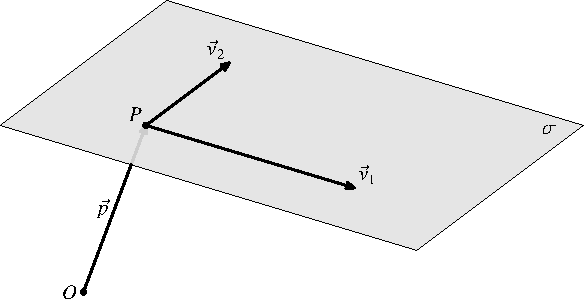
\includegraphics{images/v-8}
\end{center}
\caption{Parametrisierung einer Ebene.\label{image-parametrisierungebene}}
\end{figure}%
Ebenen zeichnen sich gegen"uber Geraden dadurch aus, dass sich auf ihr
ein Punkt nicht nur in einer Richtung, sondern unabh"angig zwei Richtungen
bewegen kann. Wir brauchen also einen zweiten Richtungsvektor, und einen
zweiten Parameter. Die Punkte einer Ebene $\sigma$ werden also beschrieben durch
\[
\vec r=\vec p+t\vec v_1+s\vec v_2,
\]
(Abbildung~\ref{image-parametrisierungebene}).

\begin{beispiel}
Man finde die Parameterdarstellung der Ebene durch die Punkte
$A=(1,2,1)$,
$B=(3,4,-1)$ und
$C=(4,-1,0)$.

\smallskip

{\parindent 0pt Die} Vektoren $\vec u=\overrightarrow{AB}$ und
$\vec v=\overrightarrow{AC}$ k"onnen als Richtungsvektoren
verwendet werden, und ergeben als Parameterdarstellung:
\begin{equation}
\vec r=\begin{pmatrix}1\\2\\1 \end{pmatrix}
+
t\begin{pmatrix}2\\2\\-2\end{pmatrix}
+
s\begin{pmatrix}3\\-3\\-1\end{pmatrix}.
\label{beispielebene}
\end{equation}
\end{beispiel}

\subsection{Durchstosspunkt\label{subsection-durchstosspunkt}}
\index{Durchstosspunkt}
\begin{figure}
\begin{center}
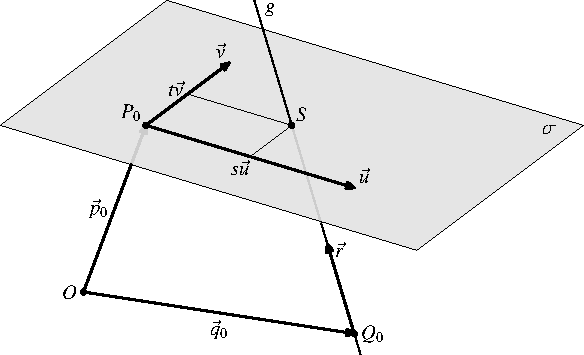
\includegraphics{images/v-9}
\end{center}
\caption{Durchstosspunkt $S$ der Geraden $g$ durch die Ebene
$\sigma$.\label{image-durchstosspunkt}}
\end{figure}
Im dreidimensionalen Raum
sind eine Gerade $g$ und eine Ebene $\sigma$ je in Parameterdarstellung gegeben, also
\begin{align*}
\sigma&=
\{
\vec p_0+s\vec u+t\vec v\;
|\;s, t\in\mathbb R\}
\\
g&=
\{
\vec q_0+l\vec r\;
|\;l\in\mathbb R
\}
\end{align*}
Es soll der Durchstosspunkt $S$ der Gerade durch die Ebene gefunden
werden (Abbildung~\ref{image-durchstosspunkt}).
Dazu m"ussen wir die Parameterwerte f"ur $s$, $t$ und $l$ finden,
f"ur die gilt
\begin{align*}
\vec p_0+s\vec u+t\vec v
&=
\vec q_0+l\vec r
\\
s\vec u+t\vec v-l\vec r&=\vec q_0+\vec p_0
\end{align*}
Dies ist eine Vektorgleichung mit den drei Unbekannten $s$, $t$ und $l$,
sie entspricht drei linearen Gleichungen f"ur diese Unbekannten.

Im Allgemeinen wird dieses Gleichungssystem genau eine L"osung haben,
n"amlich den Durchstosspunkt.
Ist die Gerade parallel zur Ebene, hat das Gleichungssystem jedoch keine
L"osung, es gibt also auch keinen Durchstosspunkt. Liegt die Gerade
dagegen in der Ebene, gibt es unendlich viele L"osungen.

In den singul"aren F"allen ist es offenbar m"oglich, die Richtung $\vec r$
der Gerade durch die beiden Vektoren $\vec u$ und $\vec v$ in der Ebene
auszudr"ucken, die drei Vektoren $\vec u$, $\vec v$ und $\vec r$ sind
linear abh"angig.

\begin{beispiel}
Finde den Durchstosspunkt der Geraden
\[
\vec r=
\begin{pmatrix} 5\\8\\3 \end{pmatrix}
+
l\begin{pmatrix} 1\\0\\1 \end{pmatrix}
\]
durch die Ebene (\ref{beispielebene}). 

\smallskip

{\parindent0pt Zusammen} mit der Gleichung (\ref{beispielebene}) bekommen wir die 
Vektorgleichung
\[
\begin{pmatrix}1\\2\\1 \end{pmatrix}
+
t\begin{pmatrix}2\\2\\-2\end{pmatrix}
+
s\begin{pmatrix}3\\-3\\-1\end{pmatrix}
=
\begin{pmatrix} 5\\8\\3 \end{pmatrix}
+
l\begin{pmatrix} 1\\0\\1 \end{pmatrix}
\quad\Rightarrow\quad
t\begin{pmatrix}2\\2\\-2\end{pmatrix}
+
s\begin{pmatrix}3\\-3\\-1\end{pmatrix}
+
l\begin{pmatrix} -1\\0\\-1 \end{pmatrix}
=
\begin{pmatrix} 4\\6\\2 \end{pmatrix}
\]
Das Gleichungssystem kann mit dem Gauss-Algorithmus
gel"ost werden
\begin{align*}
\begin{tabular}{|>{$}c<{$}>{$}c<{$}>{$}c<{$}|>{$}c<{$}|}
\hline
 2%
\begin{picture}(0,0)
\color{red}\put(-3,4){\circle{12}}
\end{picture}%
& 3&-1&4\\
 2&-3& 0&6\\
-2%
\begin{picture}(0,0)
\color{blue}\drawline(-15,-2)(-15,24)(2,24)(2,-2)
\end{picture}
&-1&-1&2\\
\hline
\end{tabular}
&
\rightarrow
\begin{tabular}{|>{$}c<{$}>{$}c<{$}>{$}c<{$}|>{$}c<{$}|}
\hline
 1& \frac32&-\frac12&2\\
 0&-6%
\begin{picture}(0,0)
\color{red}\put(-7,3){\circle{15}}
\end{picture}%
& 1&2\\
 0& 2&-2&6\\
\hline
\end{tabular}
\rightarrow
\begin{tabular}{|>{$}c<{$}>{$}c<{$}>{$}c<{$}|>{$}c<{$}|}
\hline
 1& \frac32&-\frac12&2\\
 0& 1&-\frac16&-\frac13\\
 0& 0&-\frac53%
\begin{picture}(0,0)
\color{red}\put(-7,3){\circle{16}}
\end{picture}%
&\frac{20}3\\
\hline
\end{tabular}
\\
&
\rightarrow
\begin{tabular}{|>{$}c<{$}>{$}c<{$}>{$}c<{$}|>{$}c<{$}|}
\hline
 1& \frac32&-\frac12&2\\
 0& 1&-\frac16%
\begin{picture}(0,0)
\color{blue}\drawline(-15,24)(-15,-5)(2,-5)(2,24)
\end{picture}
&-\frac13\\
 0& 0& 1&-4\\
\hline
\end{tabular}
\rightarrow
\begin{tabular}{|>{$}c<{$}>{$}c<{$}>{$}c<{$}|>{$}c<{$}|}
\hline
 1& \frac32%
\begin{picture}(0,0)
\color{blue}\drawline(-8,10)(-8,-5)(2,-5)(2,10)
\end{picture}%
& 0&0\\
 0& 1& 0&-1\\
 0& 0& 1&-4\\
\hline
\end{tabular}
\\
&
\rightarrow
\begin{tabular}{|>{$}c<{$}>{$}c<{$}>{$}c<{$}|>{$}c<{$}|}
\hline
 1& 0& 0&\frac32\\
 0& 1& 0&-1\\
 0& 0& 1&-4\\
\hline
\end{tabular}
\end{align*}
Da $l=-4$ kann man jetzt den Durchstosspunkt berechnen, er ist $S=(1,8,-1)$.
\end{beispiel}

\subsection{Schnittgerade}
\index{Schnittgerade zweier Ebenen}
\begin{figure}
\begin{center}
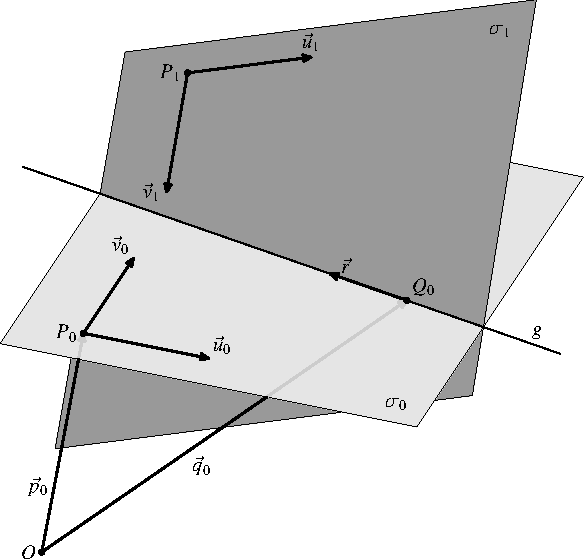
\includegraphics{images/v-10}
\end{center}
\caption{Schnittgerade $g$ zweier Ebenen $\sigma_0$ und $\sigma_1$.
\label{image-schnittgerade}}
\end{figure}
Im dreidimensionalen Raum sind zwei Ebenen
\begin{align*}
\sigma_0&=
\{\vec p_0+s_0\vec u_0+t_0\vec v_0\;|\;s_0, t_0\in\mathbb R\}
\\
\sigma_1&=
\{\vec p_1+s_1\vec u_1+t_1\vec v_1\;|\;s_1, t_1\in\mathbb R\}
\end{align*}
gegeben, gesucht ist deren Schnittgerade $g$
(Abbildung~\ref{image-schnittgerade}). Diese besteht offenbar aus
den Punkten, die sich f"ur geeignete Parameterwerte $s_0,t_0,s_1,t_1$
mit der Eigenschaft
\begin{align*}
p_0+s_0\vec u_0+t_0\vec v_0
&=
p_1+s_1\vec u_1+t_1\vec v_1
\\
s_0\vec u_0+t_0\vec v_0
-s_1\vec u_1-t_1\vec v_1
&=
-p_0+
p_1
\end{align*}
finden lassen. Dies ist ein Gleichungssystem mit drei Gleichungen f"ur
vier Unbekannte, im Allgemeinen wird sich also eine der Unbekannten
nicht bestimmen lassen, sondern die anderen Unbekannten werden sich
durch die vierte ausdr"ucken lassen. Die Punkte der Schnittmenge sind
also von der Form
\[
p_1+s_1(t_1)\vec u_1+t_1\vec v_1,
\]
wobei von der Form $s_1(t_1)=a+bt_1$ sein muss. Setzt man dies ein,
ergibt sich wieder eine Geradengleichung:
\[
p_1+s_1(t_1)\vec u_1+t_1\vec v_1
=
p_1+(a+bt_1)\vec u_1+t_1\vec v_1
=
(p_1+a\vec u_1)+t_1(b\vec u_1+v_1),
\]
eine Geradengleichung mit Richtungsvektor $\vec r = (b\vec u_1+v_1)$ und
Ausgangspunkt $\vec q_0=p_1+a\vec u_1$, also mit der Parametrisierung
\[
g=\{\vec q_0+t\vec r\;|\;t\in\mathbb R\}.
\]

\begin{beispiel}
Man finde die Schnittgerade der beiden Ebenen mit Parameterdarstellung
\[
\sigma_0:
\vec p_0+s_0\vec u_0+t_0\vec v_0
=\begin{pmatrix}5\\8\\6\end{pmatrix}
+s_0\begin{pmatrix}4\\6\\7\end{pmatrix}
+t_0\begin{pmatrix}2\\5\\6\end{pmatrix}
,
\qquad
\sigma_1:
\vec p_1+s_1\vec u_1+t_0\vec v_1
=\begin{pmatrix}5\\4\\4\end{pmatrix}
+s_1\begin{pmatrix}6\\6\\7\end{pmatrix}
+t_1\begin{pmatrix}5\\4\\4\end{pmatrix}
\]

\smallskip

{\parindent 0pt Wir setzen die beiden Parametrisierungen gleich und
erhalten}
\[
\begin{pmatrix}5\\8\\6\end{pmatrix}
+s_0\begin{pmatrix}4\\6\\7\end{pmatrix}
+t_0\begin{pmatrix}2\\5\\6\end{pmatrix}
=\begin{pmatrix}5\\4\\4\end{pmatrix}
+s_1\begin{pmatrix}6\\6\\7\end{pmatrix}
+t_1\begin{pmatrix}5\\4\\4\end{pmatrix}
\]
oder
\[
s_0\begin{pmatrix}4\\6\\7\end{pmatrix}
+t_0\begin{pmatrix}2\\5\\6\end{pmatrix}
-s_1\begin{pmatrix}6\\6\\7\end{pmatrix}
-t_1\begin{pmatrix}5\\4\\4\end{pmatrix}
=
\begin{pmatrix}0\\-4\\-2\end{pmatrix}
\]
Der Gauss-Algorithmus liefert f"ur die L"osung das Tableau
\[
\begin{tabular}{|>{$}c<{$}>{$}c<{$}>{$}c<{$}>{$}c<{$}|>{$}c<{$}|}
\hline
4&2&-6&-5& 0\\
6&5&-6&-4&-4\\
7&6&-7&-4&-2\\
\hline
\end{tabular}
\rightarrow
\begin{tabular}{|>{$}c<{$}>{$}c<{$}>{$}c<{$}>{$}c<{$}|>{$}c<{$}|}
\hline
    1&   0&   0& -\frac{11}2& -26\\
    0&   1&   0&   4&  16\\
    0&   0&   1&  -\frac32& -12\\
\hline
\end{tabular}
\]
Die Variable $t_1$ ist frei w"ahlbar, daraus lassen sich die anderen
Variablen bestimmen:
\[
\begin{linsys}{3}
s_0&=&-26&+&\frac{11}2t_1\\
t_0&=&16&-&4t_1\\
s_1&=&-12&+&\frac32t_1\\
\end{linsys}
\]
Setzt man dies in die urspr"unglichen Ebenengleichungen ein, entsteht
die Parameterdarstellung der Schnittgeraden:
\begin{align*}
\begin{pmatrix}x\\y\\z\end{pmatrix}
&=
\begin{pmatrix}5\\8\\6\end{pmatrix}
+\biggl(-26+\frac{11}2t_1\biggr)\begin{pmatrix}4\\6\\7\end{pmatrix}
+(16-4t_1)\begin{pmatrix}2\\5\\6\end{pmatrix}
=
\begin{pmatrix}-67\\-68\\-80\end{pmatrix}
+t_1
\begin{pmatrix}14\\13\\\frac{29}2\end{pmatrix},\quad\text{oder}
\\
\begin{pmatrix}x\\y\\z\end{pmatrix}
&=
\begin{pmatrix}5\\4\\4\end{pmatrix}
+\biggl(-12+\frac32t_1\biggr)\begin{pmatrix}6\\6\\7\end{pmatrix}
+t_1\begin{pmatrix}5\\4\\4\end{pmatrix}
=
\begin{pmatrix}-67\\-68\\-80\end{pmatrix}
+t_1
\begin{pmatrix}14\\13\\\frac{29}2\end{pmatrix}
\end{align*}
Nat"urlich muss man in beiden F"allen die gleiche Gerade bekommen,
dies ist eine h"ubsche Kontrolle f"ur die Richtigkeit des Resultates.
\end{beispiel}

\subsection{Vereinheitlichtes L"osungsverfahren\label{section-vereinheitlichtes-verfahren}}
Alle in den bisherigen Abschnitten vorgestellten L"osungsverfahren 
laufen darauf hinaus, dass man f"ur die Parameter der Parameterdarstellungen
Gleichungen dadurch aufstellt, dass man wo n"otig Gleichungen herstellt.
Dies ist aber eigentlich ein unn"otiger Schritt, den man auch dem
Gauss-Algorithmus "uberlassen k"onnte.

Traditionell wird das so gemacht, weil fr"uher eine grosse Angst
davor bestand, auf grosse Gleichungssysteme zu stossen, deren L"osung
m"uhsam ist. Diese Angst ist heute mit modernen Taschenrechnern und
Computer nicht mehr gerechtfertigt.

\subsubsection{Durchstosspunkt}
Um den Durchstosspunkt wie in \ref{subsection-durchstosspunkt} zu finden,
gehen wir wieder von den Parameterdarstellungen aus, schreiben jetzt
aber den gesuchten gemeinsamen Ortsvektor des Punktes
$({\color{red}x}, {\color{red}y}, {\color{red}z})$ explizit hin:
\[
\begin{pmatrix}
\color{red}x\\
\color{red}y\\
\color{red}z\\
\end{pmatrix}
=
\begin{pmatrix}1\\2\\1 \end{pmatrix}
+
{\color{red}t}\begin{pmatrix}2\\2\\-2\end{pmatrix}
+
{\color{red}s}\begin{pmatrix}3\\-3\\-1\end{pmatrix}
,\qquad
\begin{pmatrix}
\color{red}x\\
\color{red}y\\
\color{red}z\\
\end{pmatrix}
=
\begin{pmatrix} 5\\8\\3 \end{pmatrix}
+
{\color{red}l}\begin{pmatrix} 1\\0\\1 \end{pmatrix}
\]
Darin haben wir alle unbekannten Gr"ossen {\color{red}rot} markiert.
Wir haben jetzt sechs Gleichungen mit sechs Unbekannten.
Der Gauss-Algorithmus liefert direkt die L"osung, sofern es eine gibt,
ohne dass man wie in Abschnitt \ref{subsection-durchstosspunkt} 
die gefundenen Parameterwerte nochmals einsetzen m"usste:
\[
\begin{tabular}{|>{$}c<{$}>{$}c<{$}>{$}c<{$}>{$}c<{$}>{$}c<{$}>{$}c<{$}|>{$}c<{$}|}
\hline
{\color{red}x}&
{\color{red}y}&
{\color{red}z}&
{\color{red}t}&
{\color{red}s}&
{\color{red}l}&\\
\hline
1&0&0&-2&-3& 0&1\\
0&1&0&-2& 3& 0&2\\
0&0&1& 2& 1& 0&1\\
1&0&0& 0& 0&-1&5\\
0&1&0& 0& 0& 0&8\\
0&0&1& 0& 0&-1&3\\
\hline
\end{tabular}
\rightarrow
\begin{tabular}{|>{$}c<{$}>{$}c<{$}>{$}c<{$}>{$}c<{$}>{$}c<{$}>{$}c<{$}|>{$}c<{$}|}
\hline
{\color{red}x}&
{\color{red}y}&
{\color{red}z}&
{\color{red}t}&
{\color{red}s}&
{\color{red}l}&\\
\hline
1&0&0&0&0&0&1\\
0&1&0&0&0&0&8\\
0&0&1&0&0&0&-1\\
0&0&0&1&0&0&1.5\\
0&0&0&0&1&0&-1\\
0&0&0&0&0&1&-4\\
\hline
\end{tabular}
\]
Daraus liest man einerseits den Durchstosspunkt $(1,8,-1)$ ab, andererseits
findet man die Parameterwerte, f"ur die dieser Durchstosspunkt erreicht wird.

\subsubsection{Schnittgerade}
Die Schnittgerade der zwei Ebenen kann wie folgt gefunden werden.
Zun"achst beschreiben wir mit der Parameterdarstellung, wie der
Ortsvektor eines beliebigen Punktes $(x,y,z)$ der Ebenen entsteht:
\[
\begin{pmatrix}
\color{red}x\\
\color{red}y\\
\color{red}z\\
\end{pmatrix}
=
\begin{pmatrix}5\\8\\6\end{pmatrix}
+{\color{red}s_0}\begin{pmatrix}4\\6\\7\end{pmatrix}
+{\color{red}t_0}\begin{pmatrix}2\\5\\6\end{pmatrix}
,\qquad
\begin{pmatrix}
\color{red}x\\
\color{red}y\\
\color{red}z\\
\end{pmatrix}
=
\begin{pmatrix}5\\4\\4\end{pmatrix}
+{\color{red}s_1}\begin{pmatrix}6\\6\\7\end{pmatrix}
+{\color{red}t_1}\begin{pmatrix}5\\4\\4\end{pmatrix}
\]
Hier hat man pl"otzlich 6 Gleichungen f"ur 7 Unbekannte. Wir erwarten
also eine frei w"ahlbare Variable, die dann als Parameter f"ur die
Schnittgerade dienen kann. Das Gausstableau ist
\[
\begin{tabular}{|>{$}c<{$}>{$}c<{$}>{$}c<{$}>{$}c<{$}>{$}c<{$}>{$}c<{$}>{$}c<{$}|>{$}c<{$}|}
\hline
{\color{red}x}&
{\color{red}y}&
{\color{red}z}&
{\color{red}s_0}&
{\color{red}t_0}&
{\color{red}s_1}&
{\color{red}t_1}&\\
\hline
1&0&0&-4&-2& 0& 0&5\\
0&1&0&-6&-5& 0& 0&8\\
0&0&1&-7&-6& 0& 0&6\\
1&0&0& 0& 0&-6&-5&5\\
0&1&0& 0& 0&-6&-4&4\\
0&0&1& 0& 0&-7&-4&4\\
\hline
\end{tabular}
\rightarrow
\begin{tabular}{|>{$}c<{$}>{$}c<{$}>{$}c<{$}>{$}c<{$}>{$}c<{$}>{$}c<{$}>{$}c<{$}|>{$}c<{$}|}
\hline
{\color{red}x}&
{\color{red}y}&
{\color{red}z}&
{\color{red}s_0}&
{\color{red}t_0}&
{\color{red}s_1}&
{\color{red}t_1}&\\
\hline
1&0&0&0&0&0&-14 &-67\\
0&1&0&0&0&0&-13 &-68\\
0&0&1&0&0&0&-14.5&-80\\
0&0&0&1&0&0&-5.5&-26\\
0&0&0&0&1&0&4&-16\\
0&0&0&0&0&1&-1.5&-12\\
\hline
\end{tabular}
\]
Daraus liest man ab, dass es unendlich viele Punkte gibt, die auf beiden
Ebenen liegen, und dass $t_1$ als Parameter f"ur die Geradengleichung
dienen kann. Ausserdem kann man die Parameterdarstellung der Gerade ablesen:
\[
\begin{pmatrix}-67\\-68\\-80\end{pmatrix}
+t_1
\begin{pmatrix}14\\13\\14.5\end{pmatrix}.
\]
\section{Skalarprodukt}
\index{Skalarprodukt}
Abstand und Winkel spielen in der euklidischen Geometrie eine fundamentale
Rolle, die bisher eingef"uhrten Elemente der Vektorgeometrie erlauben
jedoch noch nicht, Abst"ande oder Winkel zu berechnen. Dazu ist ein neues
Konstrukt erforderlich, das Skalarprodukt.

\subsection{Orthogonale Projektion}
\index{orthogonale Projektion}
\index{Projektion!orthogonale|see{orthogonale Projektion}}
Zun"achst m"ochten wir zeigen, dass sich L"angen und Winkel berechnen
lassen, wenn man in der Lage ist, die L"ange der orthogonalen Projektion
eines Vektors auf jeden beliebigen anderen Vektor zu berechnen.
\begin{figure}
\begin{center}
\includegraphics{images/s-1}
\end{center}
\caption{Orthogonale Projektion\label{orthproj}}
\end{figure}

Seien also $\vec u$, $\vec v$ zwei beliebige Vektoren wie in Abbildung~\ref{orthproj}, und $p_{\vec u}(\vec v)$
die L"ange der Projektion des Vektors $\vec v$ auf $\vec u$.
Wir versehen diese L"ange mit einem Vorzeichen, zeigt der auf $\vec u$
projizierte Vektor $\vec v$ in die gleiche Richtung wie $\vec u$ 
nehmen wir die L"ange positiv, zeigt der projizierte Vektor in die
Gegenrichtung, ist $p_{\vec u}(\vec v)$ negativ.

Die L"ange von $\vec v$ ist $p_{\vec v}(\vec v)$, und f"ur den Winkel
$\alpha$ zwischen den beiden Vektoren ist
\begin{equation}
\cos \alpha = \frac{p_{\vec u}(\vec v)}{p_{\vec v}{\vec v}}.
\label{zwischenwinkel}
\end{equation}
Offenbar ist die L"ange der Projektion die grundlegendere Gr"osse,
aus der man die anderen Konzepte ableiten kann. Etwas ung"unstig
ist an dieser Projektion nur, dass die beiden Vektoren nicht
symmetrisch eingehen.
Immerhin ist $p_{\vec u}(\vec v)$ linear in $\vec v$, wie man
sich mit einer 
Zeichnung sofort "uberzeugen kann, es ist also
\begin{align*}
p_{\vec u}(\vec v_1+\vec v_2)&=p_{\vec u}(\vec v_1)+p_{\vec u}(\vec v_2)\\
p_{\vec u}(\lambda \vec v)&=\lambda p_{\vec u}(\vec v).
\end{align*}

\subsection{Skalarprodukt}
\index{Skalarprodukt}
\begin{figure}
\begin{center}
\includegraphics{images/s-2}
\end{center}
\caption{Skalarprodukt $\vec u\cdot \vec v$ der Vektoren $\vec u$ und $\vec v$ mit Zwischenwinkel
$\alpha$.\label{image-skalarprodukt}}
\end{figure}
Gesucht ist daher eine Konstruktion, welche immer noch linear ist,
aber auch symmetrisch in $\vec u$ und $\vec v$.
Die Formel (\ref{zwischenwinkel}) deutet auch an, wie dies erreicht
werden kann. Der Zwischenwinkel kann nat"urlich auch berechnet werden,
indem die beiden Vektoren vertauscht werden:
\[
\cos \alpha
=
\frac{p_{\vec u}(\vec v)}{p_{\vec v}(\vec v)}
=
\frac{p_{\vec v}(\vec u)}{p_{\vec u}(\vec u)}
\]
Multipliziert man diese Gleichung mit 
$
p_{\vec u}(\vec u)
p_{\vec v}(\vec v)
$, erh"alt man
\[
\vec u\cdot\vec v
=
p_{\vec u}(\vec u)
p_{\vec v}(\vec v)
\cos\alpha =
p_{\vec u}(\vec u)p_{\vec u}(\vec v)
=
p_{\vec v}(\vec v)p_{\vec v}(\vec u),
\]
was offenbar symmetrisch in $\vec u$ und $\vec v$ ist.

\begin{definition}Das Skalarprodukt zweier Vektoren $\vec u$ und
$\vec v$ ist
\[
\vec u\cdot\vec v
=
p_{\vec u}(\vec u)
p_{\vec v}(\vec v)
\cos\alpha.
\]
\end{definition}
Diese Gr"osse ist linear in $\vec u$ und linear in $\vec v$, und man kann
daraus $p_{\vec u}(\vec v)$ mittels
\[
p_{\vec u}(\vec v)
=
\frac{p_{\vec u}(\vec v)p_{\vec v}(\vec v)}{p_{\vec v}(\vec v)}
=
\frac{\vec u\cdot\vec v}{\sqrt{p_{\vec v}(\vec v)^2}}
=
\frac{\vec u\cdot\vec v}{\sqrt{\vec v\cdot \vec v}}
\]
wieder zur"uckgewinnen.

\begin{satz}
Seien $\vec u$ und $\vec v$ zwei Vektoren, dann ist
\[
|\vec u|=p_{\vec u}(\vec u)=\sqrt{\vec u\cdot\vec u}
\]
die L"ange des Vektors, und f"ur den Zwischenwinkel $\alpha$ gilt
\[
|\vec u|\,|\vec v|\cos\alpha=\vec u\cdot\vec v
\]
Zwei vom Nullvektor verschiedene Vektoren  stehen genau dann senkrecht
aufeinander, wenn $\vec u\cdot\vec v=0$.
Die Projektion $\vec v_{\|}$ von $\vec v$ auf $\vec u$ ist
\[
\vec v_{\|}=\frac{\vec v\cdot\vec u}{\vec u\cdot\vec u}\vec u.
\]
Ist $\vec u$ ein Einheitsvektor, dann ist $\vec v_{\|}=(\vec v\cdot \vec u)\vec u$.
\end{satz}
\index{Zwischenwinkel}

Zur praktischen Berechnung des Skalarproduktes ben"otigen wir
eine Formel, die das Skalarprodukt aus den Vektorkomponenten 
berechnet. Schreibt man
\[
\vec u=\begin{pmatrix}u_1\\u_2\\u_3\end{pmatrix}
=u_1\vec e_1+u_2\vec e_2+u_3\vec e_3
,
\qquad
\vec v=\begin{pmatrix}v_1\\v_2\\v_3\end{pmatrix}
=v_1\vec e_1+v_2\vec e_2+v_3\vec e_3
\]
dann kann das Skalarprodukt mit der Linearit"at berechnet werden:
\begin{align*}
\vec u\cdot\vec v
&=
(u_1\vec e_1+u_2\vec e_2+u_3\vec e_3)\cdot
(v_1\vec e_1+v_2\vec e_2+v_3\vec e_3)
\\
&=
u_1v_1\vec e_1\cdot\vec e_1+
u_1v_2\vec e_1\cdot\vec e_2+
u_1v_3\vec e_1\cdot\vec e_3\\
&\qquad +
u_2v_1\vec e_2\cdot\vec e_1+
u_2v_2\vec e_2\cdot\vec e_2+
u_2v_3\vec e_2\cdot\vec e_3\\
&\qquad+
u_3v_1\vec e_3\cdot\vec e_1+
u_3v_2\vec e_3\cdot\vec e_2+
u_3v_3\vec e_3\cdot\vec e_3
\end{align*}
Die Skalarprodukte von aufeinander senkrecht stehenden Vektoren
verschwinden, es bleiben nur die Termen mit $\vec e_i\cdot\vec e_i$,
das Skalarprodukt eines Vektors mit sich selbst ist das Quadrat
der L"ange, also $\vec e_i\cdot \vec e_i=1$ und so erhalten wir den
Satz
\begin{satz}
Das Skalarprodukt zweier Vektoren 
\[
\vec u=\begin{pmatrix}u_1\\u_2\\u_3\end{pmatrix},
\qquad
\vec v=\begin{pmatrix}v_1\\v_2\\v_3\end{pmatrix}
\]
ist
\[
\vec u\cdot\vec v
=
u_1v_1+u_2v_2+u_3v_3.
\]
\end{satz}

\begin{beispiel}
Berechne die L"ange und den Zwischenwinkel der Vektoren
\begin{align*}
\vec a&= \begin{pmatrix} 3\\12\\ 4 \end{pmatrix},
&
\vec b&= \begin{pmatrix}2\\3\\6\end{pmatrix}.
\end{align*}

\smallskip

{\parindent 0pt Die} L"ange der Vektoren ist
\begin{align*}
|\vec a|
&
=\sqrt{\vec a\cdot \vec a}
&
|\vec b|
&
=\sqrt{\vec b\cdot \vec b}
\\
&=\sqrt{9+144+16}
&
&=\sqrt{4+9+36}
\\
&=\sqrt{169}=13
&
&
=\sqrt{49}=7
\end{align*}
Damit kann man jetzt auch den Zwischenwinkel berechnen
\begin{align*}
\cos\alpha&= \frac{\vec a\cdot \vec b}{|\vec a|\;|\vec b|}
=
\frac{6+36+24}{13\cdot 7}=\frac{66}{91}=0.72527
\\
\alpha&=43.51^\circ
\end{align*}
\end{beispiel}

\subsection{Ebenen}
\begin{figure}
\begin{center}
\includegraphics{images/s-3}
\end{center}
\caption{Ebene in Normalenform\label{image-normalenform}}
\end{figure}
Das Skalarprodukt gibt uns eine neue M"oglichkeit, Ebenen zu
beschreiben.
Eine Ebene durch den Punkt $P$ senkrecht auf den Vektor
$\vec n$ besteht genau aus jenen Punkten $Q$, f"ur die der Vektor
$\overset{\rightarrow}{PQ}$ auf $\vec n$ senkrecht steht
(Abbildung~\ref{image-normalenform}). Mit dem Skalarprodukt
ausgedr"uckt: Die Menge der Ortsvektoren der Punkte einer Ebene durch $P$ mit
\index{Normale}
Normale $\vec n$ ist
\[
\{\vec r\;|\;(\vec r-\vec p)\cdot \vec n=0\}
\]
Multipliziert man die Gleichung aus, erh"alt man
\begin{align*}
\left(
\begin{pmatrix}x\\y\\z\end{pmatrix}
-\begin{pmatrix}p_1\\p_2\\p_3\end{pmatrix}\right)\cdot
\begin{pmatrix}n_1\\n_2\\n_3\end{pmatrix}&=0
\\
(x-p_1)n_1+(y-p_2)n_2+(z-p_3)n_3&=0
\\
n_1x+n_2y+n_3z&=p_1n_1+p_2n_2+p_3n_3
\end{align*}
Diese Form der Ebenengleichung, in der $\vec n$ ein Einheitsnormalenvektor ist,
heisst auch Hessesche Normalform.
\index{Normalenform}
\index{Hessesche Normalform}

\begin{satz}
Ist $\vec n$ ein Einheitsvektor, dann ist
\[
d=(\vec r-\vec p)\cdot \vec n
\]
der Abstand des Punktes mit dem Ortsvektor $\vec r$ von der Ebene durch
den Punkt mit Ortsvektor $\vec p$ und Normalen $\vec n$.
\end{satz}
\begin{proof}[Beweis]
$(\vec r-\vec p)\cdot \vec n$ ist die L"ange der Projektion des Vektors
$\vec r -\vec p$ auf den Normalenvektor $\vec n$, also genau der behauptete
Abstand.
\end{proof}

\begin{beispiel}
Man finde die Normalenform der Ebenengleichung (\ref{beispielebene}),
und berechne den Abstand des Punktes $(1,1,1)$ von der Ebene.

\medskip

{\parindent 0pt Gesucht ist ein Vektor $\vec n$, der auf beiden
Richtungsvektoren senkrecht steht, also}
\begin{equation}
\begin{pmatrix}n_1\\n_2\\n_3\end{pmatrix}
\cdot
\begin{pmatrix}2\\2\\-2\end{pmatrix}
=0,
\qquad
\begin{pmatrix}n_1\\n_2\\n_3\end{pmatrix}
\cdot
\begin{pmatrix}3\\-3\\-1\end{pmatrix}
=0
\label{gleichungen-fuer-normale}
\end{equation}
Dies ist gleichbedeutend mit dem Gleichungssystem
\[
\begin{pmatrix}
2&2&-2\\
3&-3&-1
\end{pmatrix}
\begin{pmatrix}n_1\\n_2\\n_3\end{pmatrix}
=\begin{pmatrix}0\\0 \end{pmatrix}
\]
Der Gauss-Algorithmus liefert
\begin{align*}
\begin{tabular}{|>{$}c<{$}>{$}c<{$}>{$}c<{$}|}
\hline
2%
\begin{picture}(0,0)
\color{red}\put(-3,4){\circle{12}}
\end{picture}%
&2&-2\\
3%
\begin{picture}(0,0)%
\color{blue}\drawline(-8,-2)(-8,10)(2,10)(2,-2)
\end{picture}%
&-3&-1\\
\hline
\end{tabular}
&\rightarrow
\begin{tabular}{|>{$}c<{$}>{$}c<{$}>{$}c<{$}|}
\hline
1&1&-1\\
0&-6%
\begin{picture}(0,0)%
\color{red}\put(-7,4){\circle{15}}
\end{picture}%
&2\\
\hline
\end{tabular}
\rightarrow
\begin{tabular}{|>{$}c<{$}>{$}c<{$}>{$}c<{$}|}
\hline
1&1%
\begin{picture}(0,0)
\color{blue}\drawline(-8,10)(-8,-2)(2,-2)(2,10)
\end{picture}%
&-1\\
0&1&-\frac13\\
\hline
\end{tabular}
\rightarrow
\begin{tabular}{|>{$}c<{$}>{$}c<{$}>{$}c<{$}|}
\hline
1&0&-\frac23\\
0&1&-\frac13\\
\hline
\end{tabular}
\end{align*}
Die Komponente $n_3$ ist frei w"ahlbar, wir setzen $n_3=3$, und bekommen
$n_1=2$ und $n_2=1$.
Tats"achlich ist
\begin{align*}
\begin{pmatrix}2\\1\\3\end{pmatrix}
\cdot
\begin{pmatrix}2\\2\\-2\end{pmatrix}
&=4+2-6=0
&
\begin{pmatrix}2\\1\\3\end{pmatrix}
\cdot
\begin{pmatrix}3\\-3\\-1\end{pmatrix}
&=6-3-3=0.
\end{align*}
Damit ist die Normalenform der Ebenegleichung
\begin{align}
\begin{pmatrix}2\\1\\3\end{pmatrix}\cdot\left(
\begin{pmatrix}x\\y\\z\end{pmatrix} - \begin{pmatrix}1\\2\\1\end{pmatrix}
\right)&=0\notag\\
\Rightarrow\qquad
2x+y+3z&=7\label{normalenform}
\end{align}
Diese Form ist zwar eine Normalenform, aber noch nicht die Hessesche
Normalform, da man f"ur diesen Zweck einen Einheitsvektor als
Normalenvektor verwenden muss. Unser Normalenvektor hat aber die
L"ange $|\vec n|=\sqrt{14}$. Dividieren wir die Gleichung (\ref{normalenform})
durch $\sqrt{14}$, erhalten wir die Hessesche Normalform:
\[
d=\frac{2}{\sqrt{14}}x+\frac{1}{\sqrt{14}}y+\frac{3}{\sqrt{14}}z-\frac{7}{\sqrt{14}},
\]
mit der wir jetzt den Abstand $d = (2+1+3-7)/\sqrt{14}=-1/\sqrt{14}=0.26726$
bekommen k"onnen. 
\end{beispiel}

\subsection{Spiegelung\label{spiegelung}}
\begin{figure}
\begin{center}
\includegraphics{images/s-4}
\end{center}
\caption{Spiegelung eines Vektors $\vec v$ an der Ebene senkrecht auf $\vec n$.
\label{image-spiegelung}}
\end{figure}
Da man mit dem Skalarprodukt senkrechte Projektionen berechnen kann,
muss es auch m"oglich sein, die Spiegelung eines Vektors $\vec v$
an einer Ebene mit Normale $\vec n$ zu berechnen ($|\vec n|=1$).
Dazu zerlegt man den Vektor $\vec v$ in eine Komponente $\vec v_{\|}$
parallel zur Ebene und eine Komponenten $\vec v_{\perp}$ senkrecht dazu,
also $\vec v=\vec v_{\|}+\vec v_{\perp}$ (Abbildung~\ref{image-spiegelung}).
Die senkrechte Komponente 
ist im wesentlichen die Projektion von $\vec v$ auf $\vec n$:
\[
\vec v_{\perp}=
(\vec v\cdot\vec n)\vec n
.
\]
Die parallele Komponente ist der Rest:
\[
\vec v_{\|}=\vec v -\vec v_{\perp}=
\vec v-(\vec v\cdot\vec n)\vec n
,
\]
Beim gespiegelten Vektor zeigt die senkrechte Komponente in die
entgegegengesetze Richtung:
\begin{equation}
\vec v_{\text{gespiegelt}}=
\vec v_{\|}-\vec v_{\perp}
=
\vec v-(\vec v\cdot\vec n)\vec n
-
(\vec v\cdot\vec n)\vec n
=\vec v-2(\vec v\cdot\vec n)\vec n.
\label{spiegelung}
\end{equation}

\begin{beispiel}
Man spiegle den Vektor $\vec a$ an der Ebene mit der Normalen $\vec n$,
\[
\vec a=\begin{pmatrix}1\\2\\3\end{pmatrix},
\qquad
\vec n=\begin{pmatrix}1\\1\\1\end{pmatrix}
\]

\smallskip

{\parindent 0pt Zun"achst stellen wir fest,} dass $\vec n$ noch
kein Einheitsvektor ist, dass wir stattdessen $\vec n_0=\vec n/\sqrt{3}$
verwenden m"ussen. Damit kann $\vec a$ jetzt die parallelen und orthogonalen
Komponenten zerlegt werden:
\[
\vec a_{\perp}=(\vec a\cdot\vec n_0)\vec n_0
=\frac1{\sqrt{3}} (1+2+3)\frac1{\sqrt{3}}\begin{pmatrix}1\\1\\1\end{pmatrix}
=\begin{pmatrix}2\\2\\2\end{pmatrix},
\quad
\vec a_{\|}=\begin{pmatrix} -1\\0\\1 \end{pmatrix}.
\]
Nach Formel (\ref{spiegelung}) ist
\[
\vec a'=\vec a_{\|}-\vec a_{\perp}
=
\begin{pmatrix}-1\\0\\1\end{pmatrix}-\begin{pmatrix}2\\2\\2\end{pmatrix}
=\begin{pmatrix}-3\\-2\\-1\end{pmatrix}.
\]
der gespiegelt Vektor.
\end{beispiel}

\subsection{Orthonormalbasis}
Die Vektoren $\vec e_i$ stehen senkrecht aufeinander und haben
L"ange $1$. Der Vektor
\[
\vec v
=
\begin{pmatrix}v_1\\v_2\\v_3\end{pmatrix}
\]
l"asst sich mit Hilfe des Skalarproduktes als Summe von Vielfachen
der Vektoren $\vec e_i$ schreiben.
Es ist n"amlich $v_i=\vec v\cdot\vec e_i$, also
\[
\vec v
=
\begin{pmatrix}v_1\\v_2\\v_3\end{pmatrix}
=
v_1\vec e_1
+
v_2\vec e_2
+
v_3\vec e_3
=
(\vec v\cdot \vec e_1)\vec e_1
+
(\vec v\cdot \vec e_2)\vec e_2
+
(\vec v\cdot \vec e_3)\vec e_3
\]
Dies funktioniert aber nicht nur f"ur die Vektoren $\vec e_i$.
Seien $\vec b_1$, $\vec b_2$ und $\vec b_3$ drei aufeinander senkrecht
stehende Vektoren der L"ange $1$. Mit dem Skalarprodukt kann man
dies durch
\[
\vec b_i\cdot\vec b_j=\begin{cases}
0&\qquad i\ne j\\
1&\qquad i=j
\end{cases}
\]
ausdr"ucken. Versucht man den den Vektor $\vec v$ als Linearkombination
der Vektoren $\vec b_i$ zu schreiben, also
\[
\vec v
=
v_1'\vec b_1
+
v_2'\vec b_2
+
v_3'\vec b_3
\]
Berechnet man jetzt das Skalarprodukt von $\vec v$ mit $\vec b_i$,
findet man
\begin{align*}
\vec b\cdot \vec b_i
&=
(
v_1'\vec b_1
+
v_2'\vec b_2
+
v_3'\vec b_3
)\cdot
\vec b_i
\\
&=
v_1'\vec b_1\cdot\vec b_i
+
v_2'\vec b_2\cdot\vec b_i
+
v_3'\vec b_3\cdot\vec b_i
\\
&=v_i'
\end{align*}
weil alle Skalarprodukte verschwinden ausser zwischen
zwei gleichen Vektoren.

\begin{definition} Die Koeffizienten der Einheitsmatrix
\[
\delta_{ij}=
\begin{cases}
0&\qquad i\ne j\\
1&\qquad i=j
\end{cases}
\]
heisst {\em Kronecker-Delta}.
\end{definition}

\begin{definition}
$n$ Vektoren $\vec b_i$ heissen orthonormiert, wenn gilt
\[
\vec b_i\cdot\vec b_j=\delta_{ij}.
\]
\end{definition}

\begin{satz}
Sind die Vektoren $\vec b_i$ orthonormiert, dann kann man jeden
Vektor $\vec v$ als Linearkombination der Vektoren $\vec b_i$
\[
\vec v=
(\vec v\cdot\vec b_1)\vec b_1
+
(\vec v\cdot\vec b_2)\vec b_2
+
(\vec v\cdot\vec b_3)\vec b_3
\]
schreiben. Diese Darstellung ist eindeutig.
\end{satz}

\begin{proof}[Beweis]
Es ist nur noch zu beweisen, dass es nur eine solche Darstellung als
Linearkombination gibt. G"abe es zwei Darstellungen, also
\begin{align*}
\vec v
&=
v_1'\vec b_1+
v_2'\vec b_2+
v_3'\vec b_3\\
&=
v_1''\vec b_1+
v_2''\vec b_2+
v_3''\vec b_3,
\end{align*}
k"onnen wir die Differenz bilden:
\[
0=
(v_1'-v_1'')\vec b_1
+
(v_2'-v_2'')\vec b_2
+
(v_3'-v_3'')\vec b_3
\]
Das Skalarprodukt mit $b_i$ ergibt dann
\[
0=(v_i'-v_i'')\quad\Rightarrow\quad v_i'=v_i''.
\]
Da wir $i$ beliebig w"ahlen k"onnen folgt, dass die
Koeffizienten $v_i'$ und $v_i''$ "ubereinstimmen.
\end{proof}

%\subsection{Verallgemeinertes Skalarprodukt}

%\begin{definition}
%Ein symmetrische Matrix $g_{ij}$ definiert ein allgemeines Skalarprodukt 
%$$g(x,y)=\sum_{i,j=1}^ng_{ij}x_iy_i$$
%der Vektoren 
%$$x=\begin{pmatrix}x_1\\\vdots\\x_n\end{pmatrix}\qquad\text{und}
%\qquad y=\begin{pmatrix}y_1\\\vdots\\y_n\end{pmatrix}.$$
%\end{definition}
%Das zu Beginn dieses Abschnitts definiert Skalarprodukt ist ein
%verallgemeinertes Skalarprodukt mit der Matrix $I$.

\subsection{Orthonormalisierung}
F"ur orthonormierte Vektoren ist es besonders einfach, eine Darstellung
eines beliebigen Vektors als Linearkombination zu finden. Es ist daher
sicher n"utzlich, aus einer Menge von Vektoren
$\{\vec a_1,\vec a_2,\vec a_3\}$ 
eine neue Menge von Vektoren zu konstruieren, die sich von der gegeben
m"oglichst wenig
unterscheidet, aber dennoch aus orthonormierten Vektoren besteht.

\begin{satz}[Gram-Schmidt]
\label{satz-gram-schmidt}
Seien $\{\vec a_1,\vec a_2,\vec a_3\}$ linear unabh"angige Vektoren.
Dann gibt es orthonormierte Vektoren $\{\vec b_1,\vec b_2,\vec b_3\}$ so,
dass $b_k$ aus $a_1,\dots,a_k$ linear kombiniert werden kann, f"ur jedes $k$.
Die $b_i$ lassen sich wie folgt berechnen
\begin{align*}
\vec b_1&=\frac1{|\vec a_1|}a_1\\
\vec b_2&=
\frac{
\vec a_2-(\vec a_2\cdot \vec b_1)\vec b_1
}{
|\vec a_2-(\vec a_2\cdot \vec b_1)\vec b_1|
}
\\
\vec b_3
&=
\frac{
\vec a_3-(\vec a_3\cdot \vec b_1)\vec b_1-(\vec a_3\cdot\vec b_2)\vec b_2
}{
|
\vec a_3-(\vec a_3\cdot \vec b_1)\vec b_1-(\vec a_3\cdot\vec b_2)\vec b_2
|
}
\\
&\phantom{=}\vdots\\
\vec b_k&=\frac{\vec a_k-(\vec a_k\cdot \vec b_1)\vec b_1-(\vec a_k\cdot \vec b_2)\vec b_2-\dots-(\vec a_k\cdot \vec b_{k-1})\vec b_{k-1}}{|\vec a_k-(\vec a_k\cdot \vec b_1)\vec b_1-(\vec a_k\cdot \vec b_2)\vec b_2-\dots-(\vec a_k\cdot \vec b_{k-1})\vec b_{k-1}|}
\end{align*}
Das Verfahren l"asst sich offenbar auf eine beliebige Zahl linear
unabh"angiger $n$-dimensionaler Vektoren verallgemeinern.
\end{satz}

Auf die Reihenfolge der Vektoren kommt es entscheidend an, wie die 
folgenden zwei Beispiele zeigen
\begin{beispiel}
Die Vektoren 
\[
\vec a_1=\begin{pmatrix}1\\0\\0\end{pmatrix},\qquad
\vec a_2=\begin{pmatrix}1\\1\\0\end{pmatrix},\qquad
\vec a_3=\begin{pmatrix}1\\1\\1\end{pmatrix} 
\]
sind zu orthonormieren.

Die Formeln aus Satz~\ref{satz-gram-schmidt} liefern folgende Vektoren:
\begin{align*}
\vec b_1&=\frac{\vec a_1}{|\vec a_1|}=\begin{pmatrix}1\\0\\0\end{pmatrix}\\
\vec b_2&=
\frac{
\vec a_2-(\vec a_2\cdot \vec b_1)\vec b_1
}{
|\vec a_2-(\vec a_2\cdot \vec b_1)\vec b_1|
}
=
\frac{
\begin{pmatrix}1\\1\\0\end{pmatrix}-1\cdot\begin{pmatrix}1\\0\\0\end{pmatrix}
}{\dots}=\begin{pmatrix}0\\1\\0\end{pmatrix}\\
\\
\vec b_3&=
\frac{\vec a_3 -(\vec a_3\cdot \vec b_1)\vec b_1-(\vec a_3\cdot\vec b_2)\vec b_2}{\dots}
=\frac{\begin{pmatrix}1\\1\\1\end{pmatrix}-1\cdot \begin{pmatrix}1\\0\\0\end{pmatrix}-1\cdot\begin{pmatrix}0\\1\\0\end{pmatrix}
}{\dots}=\begin{pmatrix}0\\0\\1\end{pmatrix}
\end{align*}
Man findet also genau die Vektoren der Standardbasis.
\end{beispiel}

\begin{beispiel}
Die Vektoren 
\[
\vec a_1=\begin{pmatrix}1\\0\\0\end{pmatrix},\qquad
\vec a_2=\begin{pmatrix}1\\1\\1\end{pmatrix},\qquad
\vec a_3=\begin{pmatrix}1\\1\\0\end{pmatrix} 
\]
sind zu orthonormieren.

Dieses Beispiel unterscheidet sich vom vorangegangenen nur
durch die Reihenfolge der Vektoren. Wieder k"onnen die 
Formeln von Satz~\ref{satz-gram-schmidt} angewandt werden:
\begin{align*}
\vec b_1&=\frac{\vec a_1}{|\vec a_1|}=\begin{pmatrix}1\\0\\0\end{pmatrix}
\\
\vec b_2
&=
\frac{\vec a_2-(\vec a_2\cdot \vec b_1)\vec b_1}{\dots}
=
\frac{\begin{pmatrix}1\\1\\1\end{pmatrix}-1\cdot\begin{pmatrix}1\\0\\0\end{pmatrix}}{\dots}=\frac1{\sqrt{2}}\begin{pmatrix}0\\1\\1\end{pmatrix}
\\
\vec b_3
&=
\frac{\vec a_3-(\vec a_3\cdot\vec b_1)\vec b_1-(\vec a_3\cdot\vec b_2)\vec b_2}{\dots}
=\frac{\begin{pmatrix}1\\1\\0\end{pmatrix}-1\cdot\begin{pmatrix}1\\0\\0\end{pmatrix}-\frac1{\sqrt{2}}\cdot\frac1{\sqrt{2}}\begin{pmatrix}0\\1\\1\end{pmatrix} }{\cdots}
=\frac{1}{\sqrt{2}}\begin{pmatrix}0\\1\\-1\end{pmatrix}.
\end{align*}
Die gefundenen Vektoren sind v"ollig verschiedenen von den Vektoren
im vorangegagenen Beispiel.
\end{beispiel}

\subsection{"Uberbestimmte Gleichungssysteme -- ``Least Squares''}
Bei einem "uberbestimmten Gleichungssystem, als einem Gleichungssystem
mit mehr Gleichungen als Unbekannten, kann man im allgemeinen nicht davon
ausgehen, dass es "uberhaupt eine L"osung gibt. Ein solches Gleichungssystem
hat die Form
\[
A v= b,
\]
wobei $A$ eine Matrix ist, die mehr Zeilen als Spalten hat.
In drei Dimensionen hat $v$ also zwei oder sogar nur eine Komponenten,
die Menge aller m"oglichen Vektoren $Av$ ist also eine Ebene oder
Gerade. 

\subsubsection{L"osung im Sinne kleinsten Abstandes}
Das beste, was man erwarten kann, ist ein Vektor $v_0$ so, dass
der Abstand des Punktes $ b$ von der Ebene (Gerade) bestehende
aus allen $Av$ f"ur $v=v_0$ am kleinsten wird. Dies geschieht
nat"urlich genau dann, wenn der Differenzvektor $b-Av_0$ auf
allen Vektoren von $Av$ senkrecht steht. 

Die Menge der Vektoren der Form $Av$ wird von den Spalten von $A$
aufgespannt, es gen"ugt also zu testen, ob $b-Av_0$ auf diesen
Vektoren senkrecht steht. Dazu m"ussen die Skalarprodukte von
Spalten von $A$ mit dem Vektor $b-Av_0$ verschwinden, oder
\[
A^t(b-Av_0)=0
\quad
\Rightarrow
\quad
A^tAv_0=A^tb
\]
wir haben also ein Gleichungssystem gefunden mit Matrix $A^tA$ und
rechter Seite $A^tb$, welches als L"osung den gesuchten Vektor
$v_0$ hat. $A^t$ hat so viele Zeilen wie $v$ Komponenten hat, also
handelt es sich um ein Gleichungssystem mit gleich vielen Gleichungen
wie Unbekannten, es wird im Allgemeinen eine eindeutig bestimmte
L"osung haben.

\begin{satz} Sei $A$ eine $n\times m$ Matrix und $b$ ein $n$-dimensionaler
Vektor. Eine L"osung im Sinne minimaler quadrierter Abst"ande 
$
(Av-b)\cdot(Av-b)
$
ist L"osung des Gleichungssystems
\[
A^tAv=A^tb
\]
mit $m$ Gleichungen und $m$ Unbekannten.
\end{satz}

\begin{beispiel}
Man finden den Fusspunkt des Lotes vom Punkt $P=(9,10,7)$ auf die Ebene
durch $O$, $A=(8,10,10)$ und $B=(9,13,12)$.

Der Fusspunkt des Lotes ist der Punkt der Ebene, der den geringsten
Abstand zu $P$ hat. Die Ebenengleichung ist
\[
A\begin{pmatrix}s\\t\end{pmatrix}=
\begin{pmatrix}
 8& 9\\
10&13\\
10&12
\end{pmatrix}
\begin{pmatrix}s\\t\end{pmatrix}.
\]
Gesucht wird die ``beste L"osung'' von
\[
A\begin{pmatrix}s\\t\end{pmatrix}=\begin{pmatrix}9\\10\\7\end{pmatrix}=b
\]
Dazu muss zun"achst die Matrix $A^tA$ und der Vektor $A^tb$
berechnet werden.
\[
A^tA=\begin{pmatrix}
264&322\\
322&394
\end{pmatrix}
,\qquad
A^tb=\begin{pmatrix}
242\\295
\end{pmatrix}.
\]
Daraus findet man die L"osung f"ur $s$ und $t$ numerisch zu
\[
\begin{pmatrix}s\\t \end{pmatrix}
=
\begin{pmatrix}
   1.07831\\
  -0.13253
\end{pmatrix}
\]
und durch Einesetzen in die Ebenengleichung den Ortsvektor des Fusspunktes
\[
\vec f = \begin{pmatrix}
   7.4337\\
   9.0602\\
   9.1928
\end{pmatrix}
\]
Man kann dieses Resultat daduch kontrollieren, dass man nachrechnet, ob
$\vec p-\vec f$ senkrecht auf beiden Richtungsvektoren der Ebene
steht:
\[
(\vec p-\vec f)^tA=\begin{pmatrix}
  -1.7451\cdot10^{-11}&  -2.1316\cdot 10^{-11}
\end{pmatrix},
\]
im Rahmen der Rechengenauigkeit steht die Differenz also tats"achlich auf
den Richtungsvektoren senkrecht.
\end{beispiel}

\subsubsection{``Alles in einem Schritt''}
In Abschnitt \ref{section-vereinheitlichtes-verfahren} wurde gezeigt,
wie man Schnittproblem mit nur einer Durchf"uhrung des Gaussalgorithmus
l"osen konnte. Im soeben gel"osten Problem musste man aber wieder
in mehrere Schritten vorgehen. Zuerst wurden $s$ und $t$ bestimmt,
und erst in einem zweiten Schritt konnte der Fusspunkt des Lotes
berechnet werden.

Nat"urlich ist das auch f"ur dieses Problem m"oglich, man behandelt
$x$, $y$ und $z$ einfach als zus"atzliche Variablen, die als Koordinaten
von $Av$ berechnet werden. Das Gauss-Tableau dazu ist
\[
\begin{tabular}{|>{$}c<{$}>{$}c<{$}>{$}c<{$}>{$}c<{$}|>{$}c<{$}|}
\hline
x&y&y&s\quad t&\\
\hline
1&0&0&        &0\\
0&1&0&-A   &0\\
0&0&1&        &0\\
\hline
 & & &A^tA    &A^tb\\
\hline
\end{tabular}
\]
\begin{beispiel}
F"ur das Zahlenbeispiel lautet dieses Gauss-Tableau:
\[
\begin{tabular}{|>{$}c<{$}>{$}c<{$}>{$}c<{$}>{$}c<{$}>{$}c<{$}|>{$}c<{$}|}
\hline
x&y&y&s  &  t&\\
\hline
1&0&0& -8& -9&0\\
0&1&0&-10&-13&0\\
0&0&1&-10&-12&0\\
\hline
0&0&0&264&322&242\\
0&0&0&322&394&295\\
\hline
\end{tabular}
\rightarrow
\begin{tabular}{|>{$}c<{$}>{$}c<{$}>{$}c<{$}>{$}c<{$}>{$}c<{$}|>{$}r<{$}|}
\hline
x&y&y&s  &  t&\\
\hline
1&0&0&0&0&7.4337\\
0&1&0&0&0&9.0602\\
0&0&1&0&0&9.1928\\
\hline
0&0&0&1&0&1.0783\\
0&0&0&0&1&-0.1325\\
\hline
\end{tabular}
\]
Man erh"alt also genau die bereits fr"uher gefundenen L"osungen.
\end{beispiel}

\section{Kreis und Kugel}
Da das Skalarprodukt die L"ange eines Vektors berechnet, kann man
jetzt auch die Menge der Punkte eines Kreises in der Ebene
oder einer Kugel im Raum vektoriell beschreiben, und damit Standardaufgaben
l"osen.
\subsection{Gleichungen von Kreis und Kugel}
\index{Kreis}
\index{Kugel}
Die Kugel $K(M,r)$ ist die Menge aller Punkte, die von einem festen Punkt, dem
Mittelpunkt oder Zentrum, alle den gleichen Abstand $r$ haben. In vektorieller
Form heisst dies, dass die Ortsvektoren von Punkten mit dem Ortsvektor des
Mittelpunktes eine Differenz konstanter L"ange haben. Schreiben wir $\vec m$
f"ur den Ortsvektor des Mittelpunktes, dann besteht die Kugel aus den
Punkten mit den
Ortsvektoren 
\[
K(M,r)
=
\{\vec p| \;|\vec p-\vec m|=r\}
=
\{\vec p| \;(\vec p-\vec m)\cdot(\vec p-\vec m)=r^2\}.
\]
Die zweite Form ist f"ur die L"osung konkreter Problem oft n"utzlicher.
\subsection{Durchstosspunkt einer Gerade mit einer Kugel\label{durchstosspunktkugel}}
Gesucht ist der Durchstosspunkt der Geraden 
\[
\vec p=\vec p_0+t\vec r
\]
durch die Kugel, also die Menge
\[
\{\vec p| \;|(\vec p_0+t\vec r)-\vec m|=r\}
\]
In der zweiten Form der Kugelgleichung haben wir
\begin{align*}
((\vec p_0+t\vec r)-\vec m)
\cdot
((\vec p_0+t\vec r)-\vec m)&=r^2
\\
(\vec p_0+t\vec r)
\cdot
(\vec p_0+t\vec r)
-2
(\vec p_0+t\vec r)\cdot \vec m
+\vec m\cdot\vec m&=r^2
\\
\vec p_0\cdot\vec p_0
+2t\vec p_0\cdot\vec r
+t^2\vec r\cdot\vec r
-2\vec p_0\cdot\vec m
-2t\vec r\cdot\vec m
+\vec m\cdot\vec m&=r^2
\\
t^2|\vec r|^2
+t(2\vec p_0\cdot\vec r-2\vec m\cdot\vec r)
+(\vec p_0\cdot\vec p_0-2\vec p_0\cdot\vec m+\vec m\cdot\vec m)&=r^2
\end{align*}
So erhalten wir die quadratische Gleichung f"ur den Parameter $t$
des Durchstosspunktes:
\[
|\vec r|^2t^2
+2\vec p_0\cdot(\vec p_0-\vec m)t
+|\vec p_0-\vec m|^2-r^2 =0.
\]
Indem wir die Diskriminante berechnen,  k"onnen wir eine Kriterium
daf"ur ableiten, ob die Gerade die Kugel ber"uhrt. Die Diskriminante
der quadratischen Gleichung $at^2+bt+c=0$ ist $\Delta = b^2-4ac$. In unserem
Fall wird daraus
\[
\Delta
=
4(\vec p_0\cdot(\vec p_0-\vec m))^2-
4|\vec r|^2(
|\vec p_0-\vec m|^2-r^2
)
\]
Die Diskriminante ist zum Beispiel immer positiv, wenn der St"utzpunkt
$\vec p_0$
der Gerade innerhalb der Kugel ist, also $|\vec p_0-\vec m|<r$
\subsection{Thaleskreis}
Mit dem Skalarprodukt kann man ausdr"ucken, von welchen Punkten aus
eine Strecke $AB$ unter einem rechten Winkel gesehen wird, es ist
dies die Menge der Punkte $P$ mit der Eigenschaft
\[
\overrightarrow{AP}\cdot\overrightarrow{BP}=0
\]
Unter Verwendung der Konvention, dass kleine Buchstaben f"ur die
Ortsvektoren der Punkte mit entsprechenden Grossbuchstaben stehen, ist
dies gleichbedeutend mit
\[
(\vec p-\vec a)\cdot(\vec p-\vec b)=0
\]
Ausmultiplizieren und quadratisch erg"anzen ergibt
\begin{align*}
\vec p^2-\vec p\cdot\vec b-\vec a\cdot\vec p+\vec a\cdot\vec b&=0
\\
\vec p^2-(\vec a+\vec b)\cdot \vec p+\vec a\cdot\vec b&=0
\\
\vec p^2-2\left(\frac{\vec a+\vec b}{2}\right)\cdot \vec p
+\left(\frac{\vec a+\vec b}{2}\right)^2
-\left(\frac{\vec a+\vec b}{2}\right)^2
+\vec a\cdot\vec b&=0
\\
\left(\vec p
-\frac{\vec a+\vec b}{2}\right)^2&=
\left(\frac{\vec a+\vec b}{2}\right)^2-\vec a\cdot \vec b
\\
&=
\frac{\vec a^2+2\vec a\cdot\vec b+\vec b^2-4\vec a\cdot \vec b}{4}
\\
&=
\frac{\vec a^2-2\vec a\cdot\vec b+\vec b^2}{4}
\\
\left(\vec p
-\frac{\vec a+\vec b}{2}\right)^2&=
\left(\frac{\vec a-\vec b}{2}\right)^2
\end{align*}
Diese Gleichung beschreibt einen Kreis um den Punkt $(\vec a+\vec b)/2$
mit dem Radius $|\vec a-\vec b|/2$. Dies ist der Thaleskreis.

\subsection{Tangentialebene in einem Punkt}
Die Normale auf eine Kugel ist immer parallel zum Radiusvektor. Daher kann
man die Gleichung der Tangentialebene in einem Punkt $\vec p_0$ der Kugel
sofort angeben:
\begin{satz}\label{kugeltangentialebene}
Die Tangentialebene an eine Kugel mit Mittelpunktsortsvektor
$\vec m$ und Radius  $r$ im Punkt mit Ortsektor $\vec p_0$ ist
\begin{equation}
\{\vec p\;|\;
(\vec p-\vec p_0)\cdot(\vec p_0-\vec m)=0
\}
\label{eqn-kugeltangente}
\end{equation}
\end{satz}
Diese Form (\ref{eqn-kugeltangente}) ist noch nicht optimal, man kann den
Radius nicht direkt ablesen. Addieren wir jedoch noch die Gleichung
der Kugel f"ur den Vektor $\vec p_0$, erhalten wir
\begin{align*}
(\vec p-\vec p_0)\cdot(\vec p_0-\vec m)&=0\\
(\vec p_0-\vec m)\cdot(\vec p_0-\vec m)&=r^2\\
\Rightarrow\qquad
(\vec p-\vec m)\cdot(\vec p_0-\vec m)&=r^2
\end{align*}
Die Tantentengleichung ist also die Kreisgleichung, in der man
eine Kopie von $\vec p$ durch den Ber"uhrpunkt $\vec p_0$ ersetzt
hat.

\subsection{Tangente von einem Punkt an einen Kreis}
Es sind die Gleichungen der Tangenten an einen Kreis $K(M,r)$ zu finden,
welche durchd den Punkt $P$ gehen. Die klassische Konstruktion der
Elementargeometrie verlangt, dass "uber der Strecke $MP$ der
Thaleskreis gezeichnet wird, die Schnittpunkte des Thaleskreis mit
$K(M,r)$ sind die Ber"uhrpunkte der Tangenten.

Die Tangenten sollen jetzt aber auf rein algebraische Art gefunden
werden. Das Problem w"are im wesentlich gel"ost, wenn der Ber"uhrpunkt $P_0$
mit Ortsvektor
$\vec p_0$ bekannt w"are. Dieser muss nat"urlich auf dem Kreis liegen,
also 
\[
(\vec p_0-\vec m)^2=r^2.
\]
Ausserdem muss der Punkt $P$ auf der Tangente im Punkt $P_0$ liegen,
also muss $MP_0$ senkrecht auf $PP_0$ stehen:
\begin{equation}
(\vec p_0-\vec m)\cdot(\vec p-\vec p_0)=0
\label{thalesbedingung}
\end{equation}
Damit haben wir zwei Gleichungen f"ur die beiden unbekannten Koordinaten
von $P_0$ gefunden, im Allgemeinen werden sie die Bestimmung von $\vec p_0$
erm"oglichen (Ausnahmen: $P$ im Inneren des Kreises).

Zur L"osung multiplizieren wir die zweite Gleichung noch aus
\begin{align*}
\vec p_0^2-\vec m\cdot\vec p_0-\vec p\cdot\vec p_0+\vec m\cdot\vec p&=0
\\
\vec p_0^2-\vec p_0\cdot (\vec m+\vec p)+\vec m\cdot\vec p&=0
\\
\vec p_0^2-2\vec p_0\cdot \left(\frac{\vec m+\vec p}{2}\right)+\vec m\cdot\vec p&=0
\\
\vec p_0^2-2\vec p_0\cdot \left(\frac{\vec m+\vec p}{2}\right)+
\left(\frac{\vec m+\vec p}2\right)^2
-\left(\frac{\vec m+\vec p}2\right)^2
+\vec m\cdot\vec p&=0
\\
\left(\vec p_0- \frac{\vec m+\vec p}{2}\right)^2
&=
\left(\frac{\vec m+\vec p}2\right)^2
-\vec m\cdot\vec p
\\
\left(\vec p_0- \frac{\vec m+\vec p}{2}\right)^2
&=
\left(\frac{\vec m-\vec p}2\right)^2
\end{align*}
Dies ist wieder ein Kreis mit Mittelpunkt $(\vec m+\vec p)/2$ und
Radius $|\vec m-\vec p|/2$, also wieder ein Thaleskreis. Das ist
nat"urlich nicht "uberraschend, die Bedingung (\ref{thalesbedingung})
ist ja nichts anderes als die Definition des Thaleskreises.
Die algebraische Rechnung macht also nichts anderes als die klassische
Konstruktion.
\subsection{Reflexion eines Lichtstrahls}
\begin{figure}
\begin{center}
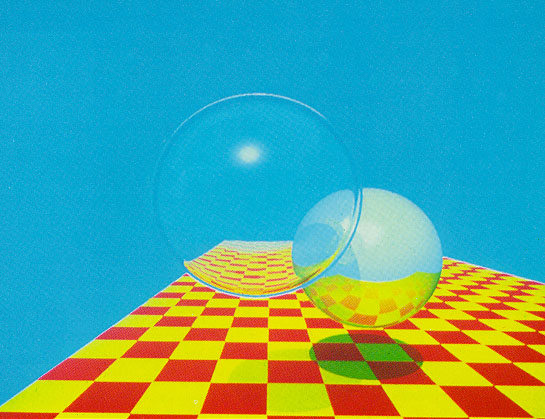
\includegraphics[width=1\hsize]{images/raytracing}
\end{center}
\caption{Mit Ray Tracing erzeugtes computergeneriertes Bild\label{raytracing}}
\end{figure}
Computergraphik-Effekte sind aus modernen Filmen nicht mehr wegzudenken.
Ganze Spielfilme wurden schon vollst"andig im Computer erzeugt.
Wie k"onnen die Bilder so realistisch wirken?

In Abschnitt \ref{spiegelung} haben wir gelernt, wie ein Vektor
gespiegelt wird. Wir k"onnen also den Lichtstrahl, der in das Auge
des Beobachters einer Szene f"allt, zur"uckverfolgen und seine Reflektion
an jeder beliebigen reflektierenden Fl"ache der Szene berechnen, bis wir bei
einer Lichtquelle oder einem nicht reflektierenden Objekt ankommen. Die
an diesem Punkt abgestrahlte Farbe ist dan jene, die der Beobachter
wahrnimmt. Dieses Verfahren nennt man Ray Tracing. Offenbar ist es sehr
aufwendig, denn Lichtstrahlen k"onnen nicht nur reflektiert, sondern auch
gestreut werden, und sie k"onnen zum Beispiel durch Nebel abgeschw"acht
werden. Die Berechnung hochaufl"osender Szenen ist daher sehr aufwendig,
die Herstellung von CG-Filmen in Spielfilm-L"ange, wie Pixar sie beispielsweise
produziert, ben"otigt die Rechenleistung grosser Computer-Cluster.

Die Berechnung der Reflexion an einer Kugel wie in Abbildung \ref{raytracing}
erfolgt nach folgendem Algorithmus:
\begin{enumerate}
\item Berechne den Durchstosspunkt des Lichtstrahles mit der reflektierenden
Kugeloberfl"ache wie in \ref{durchstosspunktkugel} beschrieben.  
\item Berechnet die Normale im Durchstosspunkt gem"ass Satz \ref{kugeltangentialebene}.
\item Berechne die gespiegelte Gerade gem"ass Abschnitt \ref{spiegelung}.
\end{enumerate}
Dieses Verfahren wird jedoch nicht nur f"ur die Computergraphik verwendet,
sondern auch in der Optik. Spiegelteleskope bestehen aus gekr"ummten Spiegeln,
durch Berechnung der Strahlen kann man erfahren, welche Abbildungsqualit"at
man von dem Teleskop erwarten kann.

\section{Vektorprodukt}
Mit dem Skalarprodukt haben wir ein Werkzeug, L"angen und Winkel zu berechnen,
es fehlt jedoch noch ein Werkzeugt, Volumina einfach zu berechnen. Orthonormierte
Vektorsysteme haben wir als sehr n"utzlich erkannt, aber die Bestimmung eines
Vektors, der auf zwei gegebenen Vektoren senkrecht steht, ist sehr kompliziert,
bisher das einzige Verfahren daf"ur ist das Orthogonalisierungsverfahren.

Dabei haben wir im Kapitel \ref{chapter-determinanten} bereits alles
bereitgestellt,
was wir f"ur die Volumenberechnung ben"otigen. Wir werden auf diesem
Weg eine neue Vektoroperation kennenlernen, das Vektorprodukt.

\subsection{Fl"acheninhalt eines Parallelogramms}
\begin{figure}
\begin{center}
\includegraphics{images/d-1}
\end{center}
\caption{Addition von Fl"acheninhalten von Parallelogrammen 
\label{image-flaeche-addition}}
\end{figure}
Zwei Vektoren $\vec u$ und $\vec v$ spannen in der Ebene ein Parallelogramm
auf. Gesucht ist der Fl"acheninhalt des Parallelogramms. Statt daf"ur eine
Formel abzuleiten, untersuchen wir zun"achst die Eigenschaften dieses
Fl"acheninhaltes in der Hoffnung, dass wir bereits ein Objekt mit den
gleichen Eigenschaften kennen.

Wir bezeichnen den Fl"acheninhalt des von $\vec u$ und $\vec v$ aufgespannten
Parallelogramms mit $A(\vec u,\vec v)$. Der Fl"acheninhalt im landl"aufigen
Sinne ist nat"urlich immer positiv, es stellt sich jedoch als
zweckm"assig heraus, wenn wir den Fl"acheninhalt hier mit einem 
Vorzeichen versehen. Und zwar soll $A(\vec u,\vec v)$ positiv sein, wenn
sich $\vec u$ mit einer Drehung von weniger als $180^\circ$ in den Vektor
$\vec v$ drehen l"asst. Wir nennen $A(\vec u, \vec v)$ den orientierten
Fl"acheninhalt.

Die Funktion $A(\vec u,\vec v)$ hat folgende Eigenschaften
\begin{itemize}
\item $A$ "andert das Vorzeichen bei Vertauschung der beiden Vektoren.
\item $A$ ist linear im ersten Argument: 
\begin{align*}
A(\vec u'+\vec u'',\vec v)&=A(\vec u',\vec v)+A(\vec v'',\vec u)
\\
A(\lambda \vec u,\vec v)&=\lambda A(\vec u,\vec v)
\end{align*}
\item Der Fl"acheninhalt eines Einheitsquadrates ist $A(\vec e_1,\vec e_2)=1$.
\end{itemize}
Die beiden Eigenschaften zusammen ergeben, dass $A$ auch linear im 
zweiten Argument ist. Im Kapitel~2 haben wir gelernt, dass es nur eine
Funktion mit diesen Eigenschaften gibt, n"amlich die Determinate:
\begin{satz}
Der orientierte Fl"acheninhalt des von den Vektoren $\vec u$ und $\vec v$
aufgespannten Parallelogramms ist
\[
A(\vec u,\vec v)=\left|\;\begin{matrix}u_1&v_1\\u_2&v_2\end{matrix}\;\right|
=u_1v_2-u_2v_1
.
\]
\end{satz}
\begin{satz}
Der Fl"acheninhalt eines Dreiecks mit den Ecken $(x_1,y_1)$, $(x_2,y_2)$ und
$(x_3,y_3)$ ist
\[
F=
\frac12\left|\;
\begin{matrix}
x_1-x_3&x_2-x_3\\
y_1-y_3&y_2-y_3\\
\end{matrix}
\;\right|
\]
\end{satz}

\begin{beispiel}
Man berechne den Fl"acheninhalt des Dreiecks mit den Ecken
$A=(1,6)$, $B=(7,5)$ und $C=(5,3)$.

\smallskip

{\parindent 0pt Die Kantenvektoren} des Dreiecks $ABC$ sind 
\[
\overrightarrow{AB}=\begin{pmatrix}6\\-1\end{pmatrix}
,\qquad
\overrightarrow{AC}=\begin{pmatrix}4\\-3\end{pmatrix}
\]
und der Fl"acheninhalt
\[
F=\frac12\left|\;\begin{matrix}
   6&  4\\
  -1& -3
\end{matrix}\;\right|=
-7
.
\]
Der Fl"acheninhalt ist also $7$.
\end{beispiel}

\subsection{Volumen eines Parallelepipeds}
\begin{figure}
\begin{center}
\includegraphics{images/d-2}
\end{center}
\caption{Addition von Volumen von Parallelepipeds\label{image-volumina}}
\end{figure}
Ganz "ahnlich kann man das Volumen eines Parallelepipeds in drei Dimensionen
berechnen, welches von drei Vektoren $\vec a$, $\vec b$ und $\vec c$
aufgespannt wird. Auch hier stellt es sich als n"utzlich heraus, 
das Volumen mit einem Vorzeichen zu versehen:
\begin{definition}
Das orientierte Volumen 
$V(\vec a,\vec b,\vec c)$
eines Parallelepipeds aufgespannt von den drei
Vektoren
$\vec a$, $\vec b$ und $\vec c$ ist positiv, wenn die drei Vektoren
eine ``rechtsh"andiges System'' bilden, also gegeneinander orientiert
sind wie die ersten drei Finger der rechten Hand, andernfalls ist
$V(\vec a,\vec b,\vec c)$ negativ.
\end{definition}
Dieses orientierte Volumen hat die folgenden Eigenschaften:
\begin{enumerate}
\item Vertauscht man zwei der drei Vektoren, "andert das Volumen das Vorzeichen.
\item $V(\vec a,\vec b,\vec c)$ ist linear im ersten Argument, wie man 
der Abbildung~\ref{image-volumina} entnehmen kann:
\begin{align*}
V(\lambda\vec a,\vec b,\vec c)
&=
\lambda V(\vec a,\vec b,\vec c)
\\
V(\vec a'+\vec a'',\vec b,\vec c)
&=
V(\vec a',\vec b,\vec c)
+
V(\vec a'',\vec b,\vec c)
\end{align*}
\item Das orientierte Volumen des Einheitsw"urfels ist
$V(\vec e_1,\vec e_2,\vec e_3)=1$.
\end{enumerate}
Aus den ersten beiden Eigenschaften k"onnen wir folgern, dass das orientierte
Volumen auch in allen anderen Argumenten linear ist.
Und wie im vorangegangenen Abschnitt schliessen wir,
dass $V(\vec a,\vec b,\vec c)$ die Determinante ist:
\begin{satz}
Das orientierte Volumen $V(\vec a,\vec b,\vec c)$ eines von den Vektoren
$\vec a$, $\vec b$ und $\vec c$ aufgespannten Parallepipeds  ist
\[
V(\vec a,\vec b,\vec c)=\left|\;\begin{matrix}
a_1&b_1&c_1\\
a_2&b_2&c_2\\
a_3&b_3&c_3\\
\end{matrix}\;\right|.
\]
\end{satz}

\begin{beispiel}
Man finde alle Parallelepipeds mit folgenden Eigenschaften:
\begin{compactenum}
\item Zwei Kanten sind $\vec a=\overrightarrow{OA}$ und $\vec b=\overrightarrow{OB}$ 
mit $A=(4,1,3)$ und $B=(5,1,2)$.
\item Die dritte Kante ist $\overrightarrow{OC}$, wobei $C$ auf der
Ebene durch $O$ mit der Normalen 
\[
\vec n=\begin{pmatrix}1\\1\\1\end{pmatrix}
\]
liegt.
\item Zwei Kanten stehen senkrecht aufeinander.
\item Das Volumen ist $8$.
\end{compactenum}

\smallskip

{\parindent 0pt Wir suchen einen Vektor}
\[
\vec c=\begin{pmatrix}x\\y\\z\end{pmatrix},
\]
der die Bedingungen der Aufgabe erf"ullt. Zun"achst muss $\vec c$ auf
$\vec n$ senkrecht stehen, also $\vec c\cdot\vec n=0$ oder
\[
x+y+z=0.
\]
Da $\vec a\cdot\vec b=20+1+6=27\ne 0$ stehen $\vec a$ und $\vec b$
nicht senkrecht, es ist also der gesuchte Vektor $\vec c$ der auf den bereits
bekannten Kanten senkrecht stehen muss.
Wir versuchen es zun"achst
mit $\vec a$, weitere L"osungen ergeben sich, wenn man stattdessen $\vec b$
verwendet.
Dies liefert die Bedingung $\vec a\cdot\vec c=0$ oder
\[
4x+y+3y=0
\]
Das Volumen kann mit der Determinante berechnet werden:
\[
V=\left|\;
\begin{matrix}
4&5&x\\
1&1&y\\
3&2&z
\end{matrix}
\;\right|=
4z+15y+2x-3x-8y-5z=-x+7y-z=\pm8.
\]
Jetzt kann der Vektor $\vec c$ mit dem Gauss-Algorithmus bestimmt werden
\begin{align*}
\begin{tabular}{|>{$}c<{$}>{$}c<{$}>{$}c<{$}|>{$}c<{$}|}
\hline
1%
\begin{picture}(0,0)
\color{red}\put(-3,4){\circle{12}}
\end{picture}%
&1&1&0\\
-1&7&-1&\pm8\\
4%
\begin{picture}(0,0)%
\color{blue}\drawline(-12,-2)(-12,24)(4,24)(4,-2)
\end{picture}%
&1&3&0\\
\hline
\end{tabular}
&
\rightarrow
\begin{tabular}{|>{$}c<{$}>{$}c<{$}>{$}c<{$}|>{$}c<{$}|}
\hline
1&1&1&0\\
0&8%
\begin{picture}(0,0)
\color{red}\put(-3,4){\circle{12}}
\end{picture}%
&0&\pm8\\
0&-3%
\begin{picture}(0,0)%
\color{blue}\drawline(-15,-2)(-15,10)(1,10)(1,-2)
\end{picture}%
&-1&0\\
\hline
\end{tabular}
\rightarrow
\begin{tabular}{|>{$}c<{$}>{$}c<{$}>{$}c<{$}|>{$}c<{$}|}
\hline
1&1&1&0\\
0&1&0%
\begin{picture}(0,0)%
\color{blue}\drawline(-8,24)(-8,-2)(2,-2)(2,24)
\end{picture}%
&\pm1\\
0&0&-1%
\begin{picture}(0,0)
\color{red}\put(-7,4){\circle{15}}
\end{picture}%
&\pm3\\
\hline
\end{tabular}
\\
&
\rightarrow
\begin{tabular}{|>{$}c<{$}>{$}c<{$}>{$}c<{$}|>{$}c<{$}|}
\hline
1&1%
\begin{picture}(0,0)%
\color{blue}\drawline(-8,10)(-8,-2)(2,-2)(2,10)
\end{picture}%
&0&\pm3\\
0&1&0&\pm1\\
0&0&1&\mp3\\
\hline
\end{tabular}
\rightarrow
\begin{tabular}{|>{$}c<{$}>{$}c<{$}>{$}c<{$}|>{$}c<{$}|}
\hline
1&0&0&\pm 2\\
0&1&0&\pm1\\
0&0&1&\mp3\\
\hline
\end{tabular}
\end{align*}
Es folgt $C=(\mp 4,\pm1,\pm3)$. Zwei weitere L"osungen findet
man auf die gleiche Weise, indem man statt der Bedingung $\vec a\cdot\vec c=0$
verlangt, dass $\vec b\cdot\vec c=0$, man findet dann
\begin{align*}
\begin{tabular}{|>{$}c<{$}>{$}c<{$}>{$}c<{$}|>{$}c<{$}|}
\hline
1%
\begin{picture}(0,0)
\color{red}\put(-3,4){\circle{12}}
\end{picture}%
&1&1&0\\
-1&7&-1&\pm8\\
5%
\begin{picture}(0,0)%
\color{blue}\drawline(-12,-2)(-12,24)(4,24)(4,-2)
\end{picture}%
&1&2&0\\
\hline
\end{tabular}
&
\rightarrow
\begin{tabular}{|>{$}c<{$}>{$}c<{$}>{$}c<{$}|>{$}c<{$}|}
\hline
1&1&1&0\\
0&8%
\begin{picture}(0,0)
\color{red}\put(-3,4){\circle{12}}
\end{picture}%
&0&\pm8\\
0&-4%
\begin{picture}(0,0)%
\color{blue}\drawline(-15,-2)(-15,10)(1,10)(1,-2)
\end{picture}%
&-3&0\\
\hline
\end{tabular}
\rightarrow
\begin{tabular}{|>{$}c<{$}>{$}c<{$}>{$}c<{$}|>{$}c<{$}|}
\hline
1&1&1&0\\
0&1&0%
\begin{picture}(0,0)
\color{blue}\drawline(-8,24)(-8,-2)(2,-2)(2,24)
\end{picture}%
&\pm1\\
0&0&-3%
\begin{picture}(0,0)
\color{red}\put(-7,4){\circle{15}}
\end{picture}%
&\pm4\\
\hline
\end{tabular}
\\
&
\rightarrow
\begin{tabular}{|>{$}c<{$}>{$}c<{$}>{$}c<{$}|>{$}c<{$}|}
\hline
1&1%
\begin{picture}(0,0)
\color{blue}\drawline(-8,10)(-8,-2)(2,-2)(2,10)
\end{picture}%
&0&\pm\frac43\\
0&1&0&\pm1\\
0&0&1&\mp\frac43\\
\hline
\end{tabular}
\rightarrow
\begin{tabular}{|>{$}c<{$}>{$}c<{$}>{$}c<{$}|>{$}c<{$}|}
\hline
1&0&0&\pm\frac13\\
0&1&0&\pm1\\
0&0&1&\mp\frac43\\
\hline
\end{tabular}
\end{align*}
also
$C=(\pm\frac13,\pm1,\mp\frac43)$.
\end{beispiel}

\subsection{Vektorprodukt}
Wir schreiben das Spatvolumen nach der Sarrusschen Regel aus:
\begin{align*}
V(\vec a,\vec b,\vec c)&=\det(\vec a,\vec b,\vec c)\\
&=
a_1b_2c_3+b_1c_2a_3+c_1a_2b_3
-a_3b_2c_1-b_3c_2a_1-c_3a_2b_1\\
&=
(a_2b_3-a_3b_2)c_1+(a_3b_1-a_1b_3)c_2+(a_1b_2-a_2b_1)c_3
\\
&=
\begin{pmatrix}
a_2b_3-a_3b_2\\
a_3b_1-a_1b_3\\
a_1b_2-a_2b_1
\end{pmatrix}
\cdot
\begin{pmatrix}
c_1\\c_2\\c_3
\end{pmatrix}
\end{align*}
Es gibt also einen Vektor $\vec a\times\vec b$, der die Berechnung
des Spatvolumens mit einem Skalarprodukt erlaubt:
\begin{definition}
Der Vektor
\[
\vec a\times\vec b= \begin{pmatrix}
a_2b_3-a_3b_2\\
a_3b_1-a_1b_3\\
a_1b_2-a_2b_1
\end{pmatrix}
\]
heisst das Vektorprodukt von $\vec a$ und $\vec b$. Die Komponenten $p_i$
des Vektorproduktes $\vec p=\vec a\times \vec b$ sind
\[
p_1
=
\left|\;\begin{matrix}
a_2&b_2\\a_3&b_3
\end{matrix}\;\right|\\
,\qquad p_2=
\left|\;\begin{matrix}
a_3&b_1\\a_1&b_3
\end{matrix}\;\right|\\
,\qquad p_3=
\left|\;\begin{matrix}
a_1&b_2\\a_2&b_1
\end{matrix}\;\right|.
\]
\end{definition}
Das Vektorprodukt hat die folgenden Eigenschaften.
\begin{satz}
Sind $\vec a$ und $\vec b$ zwei dreidimensionale Vektoren, dann gilt
\begin{itemize}
\item $\vec a\times\vec b$ steht senkrecht auf $\vec a$ und $\vec b$.
\item $|\vec a\times\vec b|$ ist der Fl"acheninhalt des von 
$\vec a$ und $\vec b$ aufgespannten Parallelogrammes im Raum
\item Ist $\alpha$ der Winkel zwischen $\vec a$ und $\vec b$, dann
ist
\[
|\vec a\times\vec b|=|\vec a|\,|\vec b|\sin \alpha.
\]
\end{itemize}
\end{satz}
\begin{proof}[Beweis]
Sei $\vec c$ ein Vektor in der von $\vec a$ und $\vec b$ aufgespannten
Ebene. In diesem Fall degeneriert das Parallelepiped, es hat Volumen $0$,
also $V(\vec a,\vec b,\vec c)= 0$.
Da also
\[
V(\vec a,\vec b,\vec c)=(\vec a\times \vec b)\cdot \vec c=0,
\]
steht $\vec c$ senkrecht auf $\vec a\times\vec b$. Da dies f"ur jeden
Vektor $\vec c$ in der von $\vec a$ und $\vec b$ aufgespannten Ebene
gilt, steht $\vec a\times\vec b$ senkrecht auf dieser Ebene, und insbesondere
auf $\vec a$ und $\vec b$. Dies beweist die Aussage a).

Sei $\vec n$ der Normalenvektor mit L"ange $1$ auf der von $\vec a$ und
$\vec b$ aufgespannten Ebene. Das Volumen $V(\vec a,\vec b,\vec n)$ ist
dasjenige eines geraden Prismas mit dem von $\vec a$ und $\vec b$
aufgespannten Prisma mit H"ohe $1$, also gleich gross wie der
Fl"acheninhalt des von $\vec a$ und $\vec b$ aufgespannten Parallelogramms.
Andererseits ist
\[
V(\vec a,\vec b,\vec n)=(\vec a\times\vec b)\cdot \vec n
\]
die Projektion des Vektors $\vec a\times\vec b$ auf $\vec n$. Die beiden
Vektoren haben aber die gleiche Richtung, weil sie beide senkrecht stehen
auf der von $\vec a$ und $\vec b$ aufgespannten Ebene. Also ist die Projektion
gerade die L"ange des Vektors, also ist
$|\vec a\times\vec b|$ der Fl"acheninhalt des Parallelogramms.

Die H"ohe des von $\vec a$ und $\vec b$ aufgespannten Parallelogramms 
ist $|\vec b|\sin \alpha$, der Fl"acheninhalt also
$|\vec a\times\vec b|=|\vec a|\,|\vec b|\sin\alpha.$
\end{proof}

\begin{beispiel}
Man bestimme das Vektorprodukt von
\[
\vec a=\begin{pmatrix}1\\2\\3\end{pmatrix} 
\quad\text{und}\quad
\vec b=\begin{pmatrix}8\\5\\13\end{pmatrix}.
\]

\smallskip
{\parindent 0pt Wir verwenden direkt die Definition}
\[
\vec a\times \vec b=
\begin{pmatrix}1\\2\\3\end{pmatrix} 
\times
\begin{pmatrix}8\\5\\13\end{pmatrix}
=
\begin{pmatrix}
2\cdot 13-3\cdot 5\\
3\cdot 8-1\cdot 13\\
1\cdot 5-2\cdot 8
\end{pmatrix}
=
\begin{pmatrix}
11\\
11\\
-11
\end{pmatrix}.
\]
\end{beispiel}

\subsection{Normale}
Das Vektorprodukt erlaubt uns jetzt auf einfache Weise die Normale einer
Ebene zu finden. Sei 
\[
\vec r=\vec p+t\vec u+s\vec v
\]
die Parameterdarstellung einer Ebene, dann ist
\[
\vec n=\vec u\times\vec v
\]
eine Normale, also ist
\[
(\vec r-\vec p)\cdot (\vec u\times\vec v)=0
\]
die implizite Form der Ebenengleichung.

\begin{beispiel}
Man finde die Normale der Ebene mit der Gleichung (\ref{beispielebene}).

\smallskip
{\parindent 0pt Die Normale haben wir schon einmal mit Hilfe der Gleichungen
(\ref{gleichungen-fuer-normale}) berechnet, jetzt kann dies
mit Hilfe des vereinfacht werden:}
\begin{equation}
\vec n = \vec u\times \vec v=
\begin{pmatrix}2\\2\\-2\end{pmatrix}
\times
\begin{pmatrix}3\\-3\\-1\end{pmatrix}
=
\begin{pmatrix}
2\cdot(-1)-(-2)\cdot(-3)\\
(-2)\cdot 3-2\cdot (-1)\\
2\cdot(-3)-2\cdot 3
\end{pmatrix}
=
\begin{pmatrix}
-8\\
-4\\
-12
\end{pmatrix}
=-4\begin{pmatrix}2\\1\\3\end{pmatrix}.
\label{beispielvektorprodukt}
\end{equation}
also ein Vielfaches des mit den Gleichungen (\ref{gleichungen-fuer-normale})
gefundenen Normale. Damit wird die Ebenengleichung
\begin{align*}
0=
\begin{pmatrix} -8\\ -4\\ -12 \end{pmatrix}\cdot
\left(
\begin{pmatrix}x\\y\\z\end{pmatrix}
-
\begin{pmatrix}1\\2\\1 \end{pmatrix}
\right)
&=
-8x-4y-12z+
28
\\
\Rightarrow
2x+y+3z&=7.
\end{align*}
\end{beispiel}

\subsection{Weitere Anwendungen}

\subsubsection{Zwischenwinkel}
F"ur den Zwischenwinkel zweier Vektoren gilt
\[
\sin\alpha=\frac{|\vec a\times\vec b|}{|\vec a|\,|\vec b|}.
\]
\begin{beispiel}
Berechne den Zwischenwinkel der Richtungsvektoren der Ebenengleichung
\ref{beispielebene}.

\smallskip

{\parindent 0pt Das Vektorprodukt der beiden Vektoren wurde
in (\ref{beispielvektorprodukt}) schon
berechnet.} Die L"ange der Vektoren ist
\[
|\vec u|=\sqrt{4+4+4}=2\sqrt{3}
,
\quad
|\vec v|=\sqrt{9+9+1}=\sqrt{19}.
\]
Die Zwischenwinkelformel liefert jetzt
\begin{align*}
\sin\alpha&=\frac{|\vec u\times \vec v|}{|\vec u|\cdot |\vec v|}
=\frac{\sqrt{64+16+144}}{\sqrt{12\cdot 19}}
=\frac{\sqrt{224}}{\sqrt{228}}=0.98246\\
\alpha&=79.252^\circ.
\end{align*}
\end{beispiel}

\subsubsection{Abstand Punkt--Gerade}
\begin{figure}
\begin{center}
\includegraphics{images/d-3}
\end{center}
\caption{Abstand Punkt--Gerade mit dem Vektorprodukt\label{punkt-gerade}}
\end{figure}
Es ist der Abstand eines Punktes mit Ortsvektor $\vec a$ von der
Geraden durch den Punkt mit Ortsvektor $\vec p$ und Richtungs $\vec r$,
also mit der Parameterdarstellung
\[
\vec q=\vec p+t\vec r
\]
zu bestimmen.
Der gesuchte Abstand $d$ ist die H"ohe des Parallelogramms,
welches von $\vec a-\vec p$
und $\vec r$ aufgespannt wird, wobei $\vec r$ als Grundseite zu betrachten ist. Der
Fl"acheninhalt $A$ des Parallelogramms kann mit dem Vektorprodukt berechnet werden:
\begin{align*}
A&=|(\vec a-\vec p)\times\vec r|\\
d&=\frac{|(\vec a-\vec p)\times\vec r|}{|\vec r|}.
\end{align*}
\subsubsection{Abstand zweier windschiefer Geraden}
\begin{figure}
\begin{center}
\includegraphics{images/d-4}
\end{center}
\caption{Abstand windschiefer Geraden\label{windschief}}
\end{figure}
Zwei nicht parallele Geraden $g_0$ und $g_1$ im Raum,
die sich nicht schneiden, heissen
{\em windschief}. 
\index{windschief}
Sie haben
einen k"urzesten Abstand $d$, der auf beiden Geraden senkrecht steht.
Sind
\begin{align*}
g_0:
\vec p&=\vec p_0+t\vec r_0\\
g_1:
\vec p&=\vec p_1+t\vec r_1
\end{align*}
Parameterdarstellungen der Geraden, dann ist die Richtung des k"urzesten
Abstandes die Richtung des Vektorproduktes $\vec n = \vec r_0\times\vec r_1$. 
Ein Vektor zwischen zwei beliebigen Punkten auf den beiden Geraden,
zum Beispiel zwischen $P_0$ und $P_1$, also der Vektor $\vec p_1-\vec p_0$,
wird als Projektion auf die Richtung des k"urzesten Abstandes immer die
L"ange dieses k"urzesten Abstandes haben. Die Projektion kann mit dem
Skalarprodukt berechnet werden, der k"urzeste Abstand $d$ ist
\[
d=(\vec p_0-\vec p_1)\cdot\frac{\vec r_0\times\vec r_1}{|\vec r_0\times\vec r_1|}.
\]

